\documentclass[aspectratio=169]{beamer}
\setbeamertemplate{navigation symbols}{}
\usepackage{color,amsmath,comment, subfigure}
\usepackage{booktabs}



%%%%%%%%%%%%%%%%%%%%%%%%%%
\title[]{Lecture 19: Social media and society}
\author[]{Matthew J. Salganik}
\institute[]{Sociology 204: Social Networks\\Princeton University}
\date[]{
1/2 What's happening on social media?
\vfill

\begin{flushleft}
\vspace{0.6in}

\includegraphics[width=0.1\textwidth]{figures/cc.png}
\end{flushleft}
}

\begin{document}
%%%%%%%%%%%%%%%%%%%%%%%%%%%
\frame{\titlepage}
%%%%%%%%%%%%%%%%%%%%%%%%%%%
\begin{frame}

\begin{itemize}
\item What is going viral?  Lies and outrage \pause
\item Who is more responsible algorithms or people?  Hard to say \pause
\item I'll try to mix in some other studies that help put these results in context.
\end{itemize}


\note{
Most focused on people: Vosoughi et al.
In between: Bradey et al.
Most focussed on algorithms: Bakshy et al.
}

\end{frame}
%%%%%%%%%%%%%%%%%%%%%%%%%%%%
\begin{frame}

Background 

\end{frame}
%%%%%%%%%%%%%%%%%%%%%%%%%%%%
\begin{frame}

\begin{center}
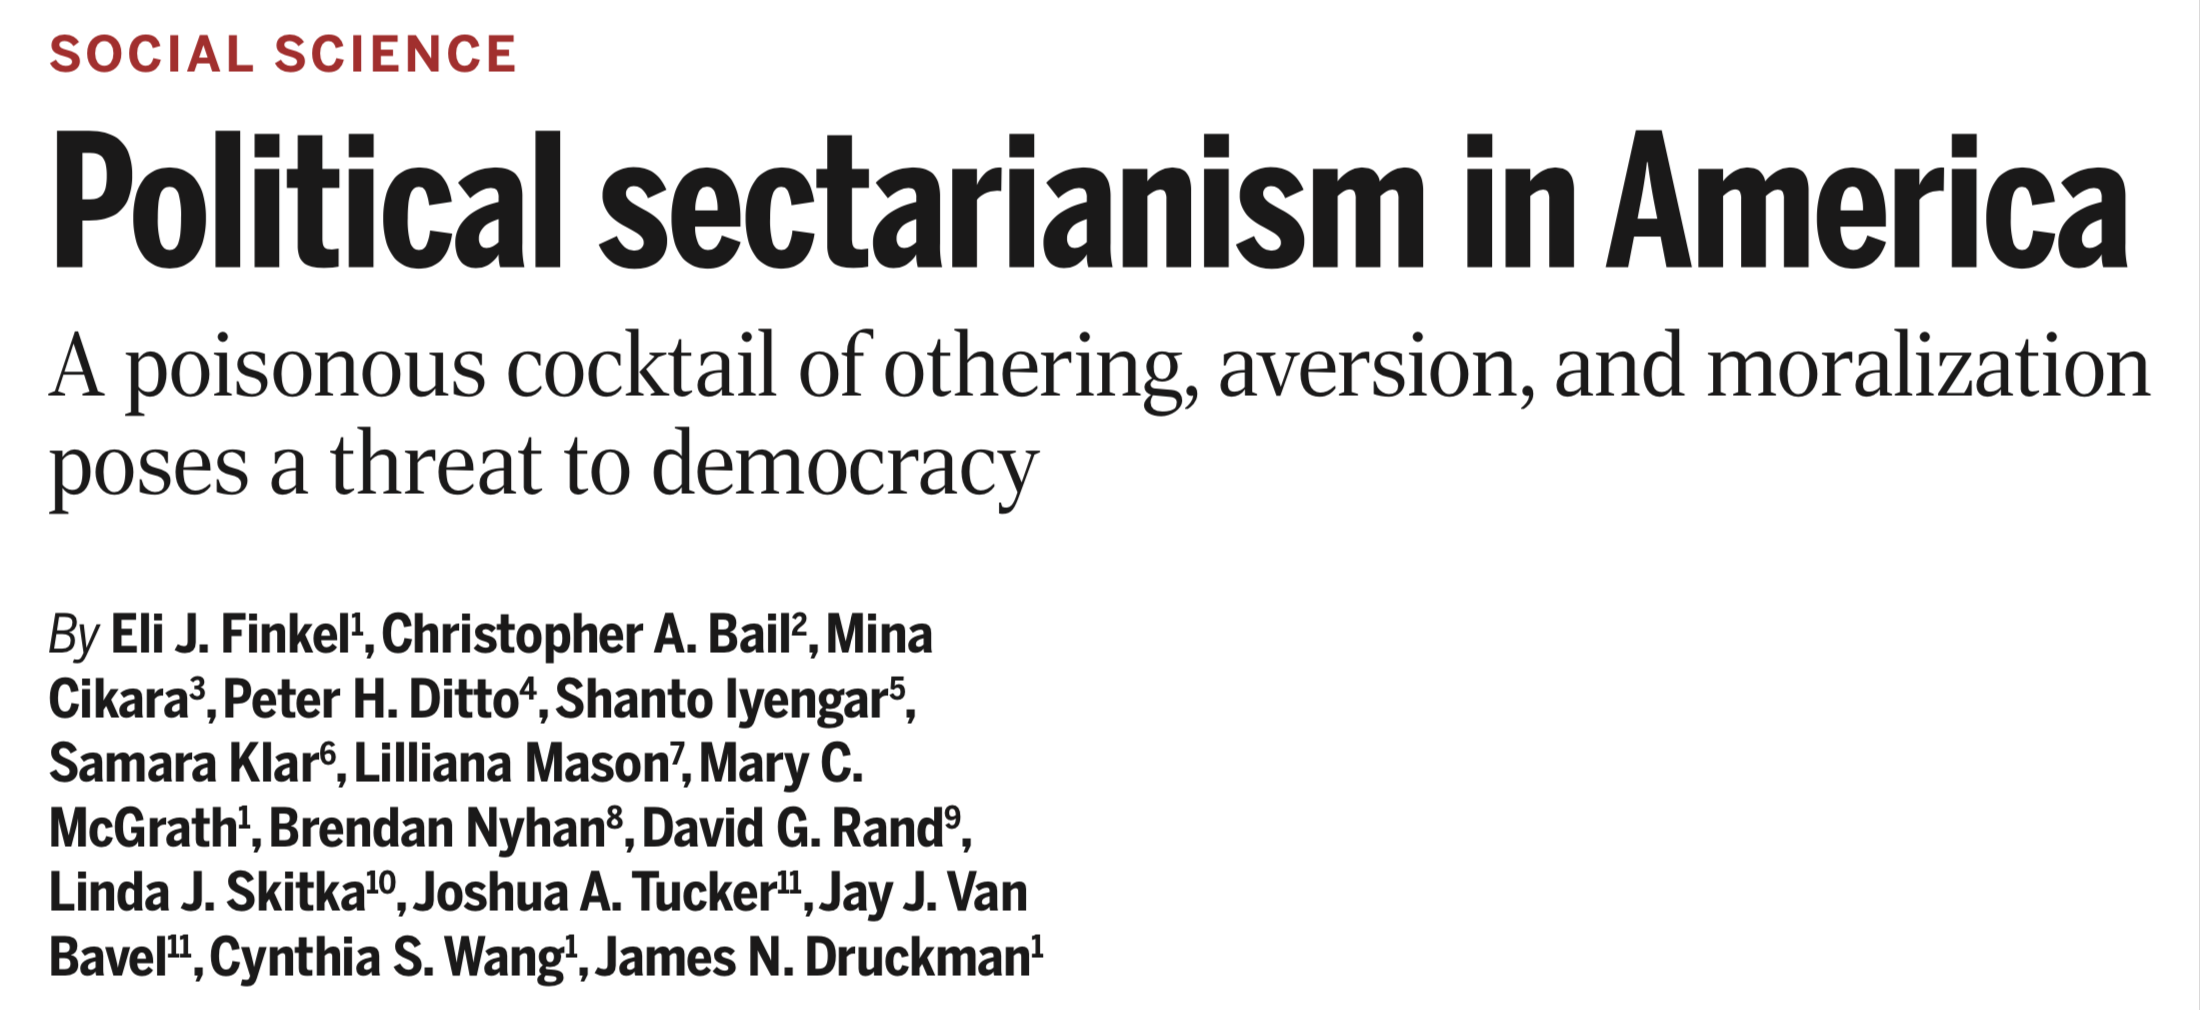
\includegraphics[width=0.95\textwidth]{figures/finkel_political_2020_title}
\end{center}

\end{frame}
%%%%%%%%%%%%%%%%%%%%%%%%%%%%%
\begin{frame}

\begin{center}
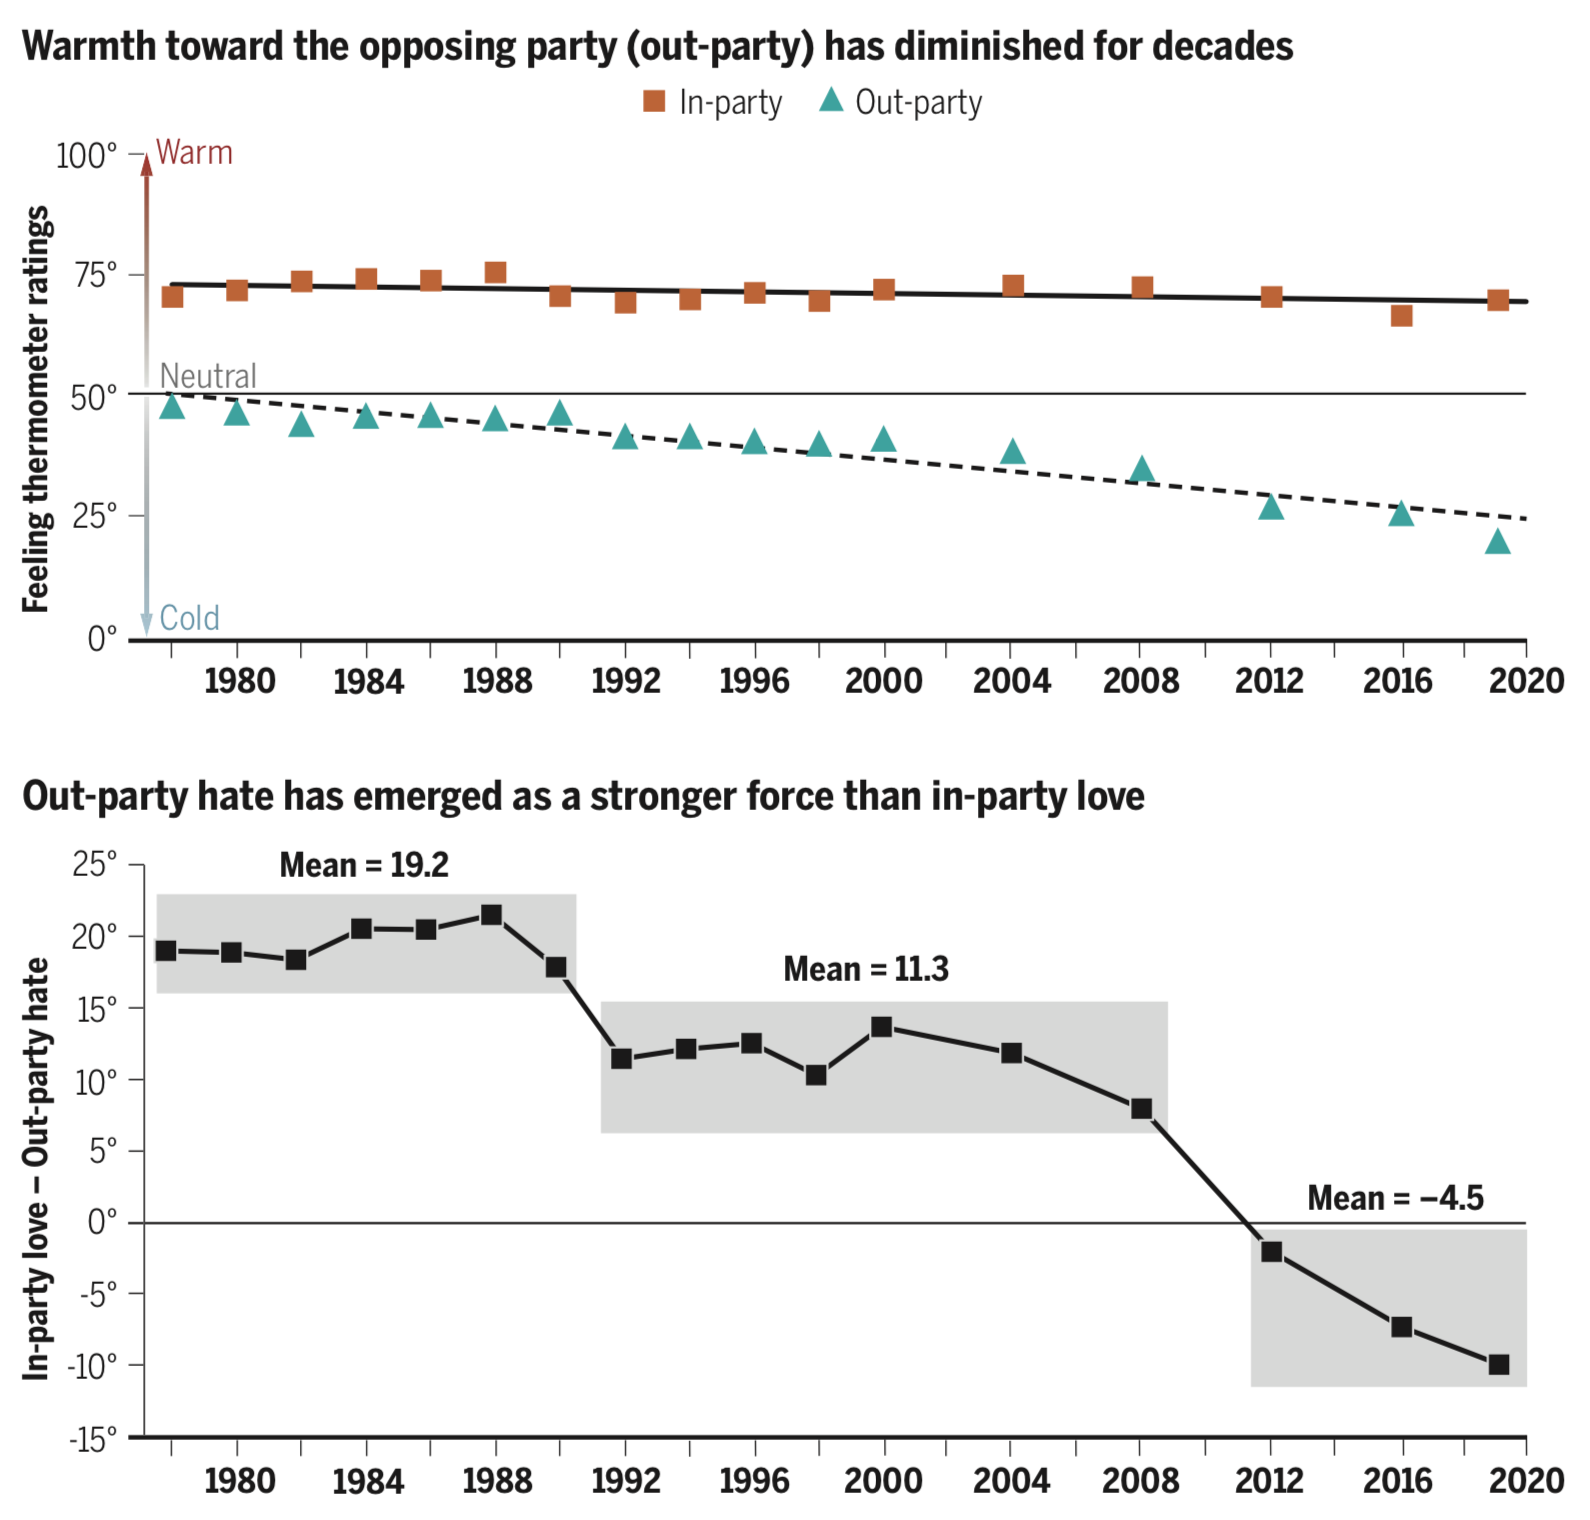
\includegraphics[height=0.95\textheight]{figures/finkel_political_2020_fig1}
\end{center}

\end{frame}
%%%%%%%%%%%%%%%%%%%%%%%%%
\begin{frame}

\begin{center}
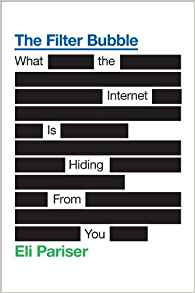
\includegraphics[height=0.95\textheight]{figures/pariser_filter_2011_cover}
\end{center}

\end{frame}
%%%%%%%%%%%%%%%%%%%%%%%%%
\begin{frame}

What goes viral? Moral outrage and lies

\end{frame}
%%%%%%%%%%%%%%%%%%%%%%%%%
\begin{frame}

\begin{center}
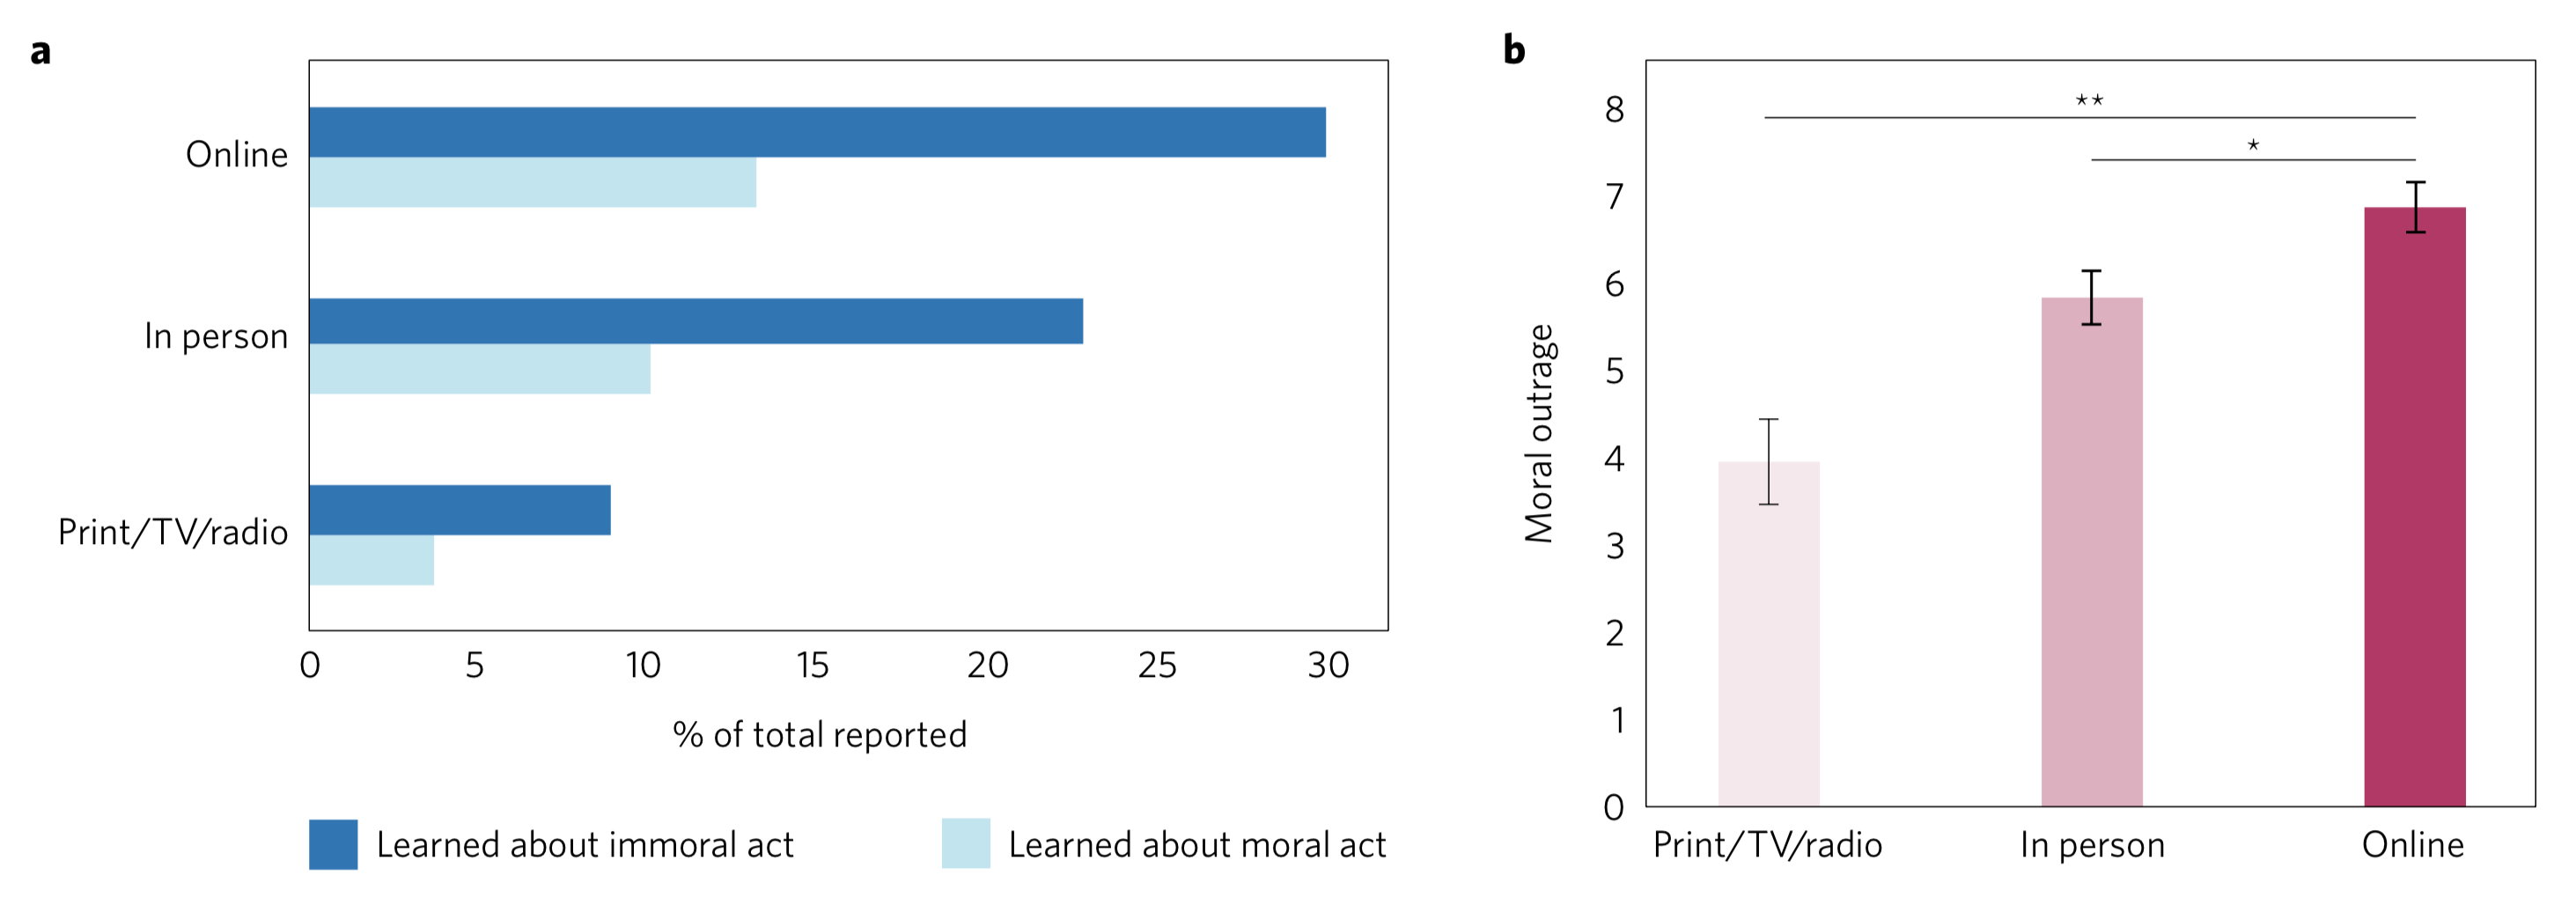
\includegraphics[width=0.95\textwidth]{figures/crockett_moral_2017_fig2}
\end{center}

\begin{itemize}
\item People more likely to learn about immoral acts online than through other media \pause
\item Outrageous acts that people see online lead to more outrage \pause
\item ``Digital media transform moral outrage by changing both the nature and prevalence of the stimuli that trigger it.''
\end{itemize}

\end{frame}
%%%%%%%%%%%%%%%%%%%%%%%%%
\begin{frame}

\begin{center}
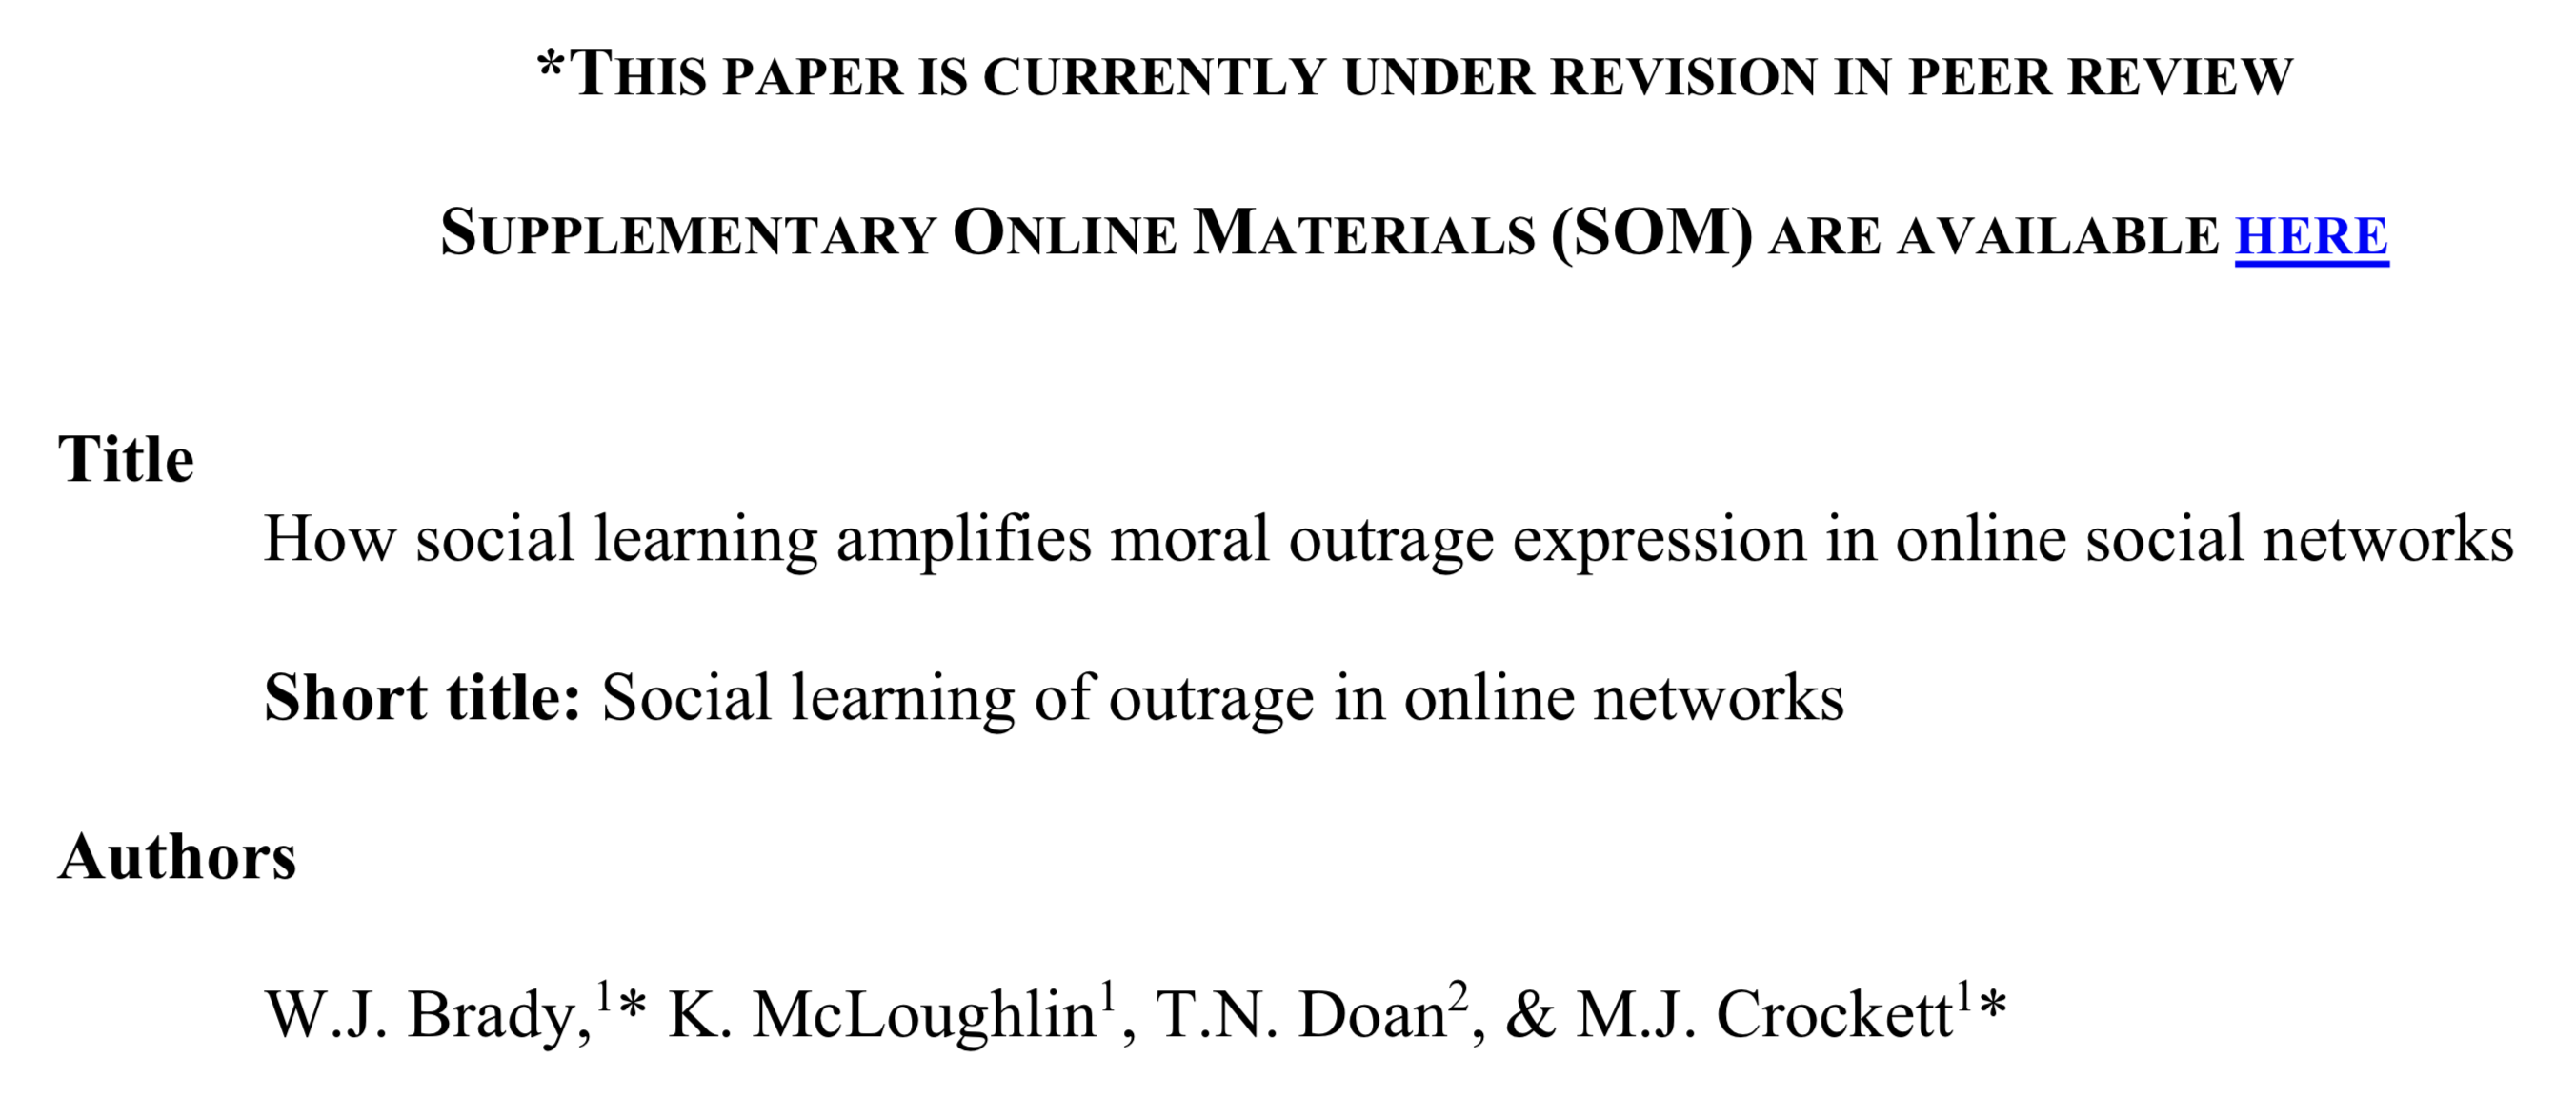
\includegraphics[width=0.95\textwidth]{figures/brady_how_2021_title}
\end{center}

\begin{itemize}
\item two observational studies and two experiments (all preregistered) \pause
\item reinforcement learning and norm learning, both of which are controlled in part by design of social media platforms
\end{itemize}

\end{frame}
%%%%%%%%%%%%%%%%%%%%%%%%%
\begin{frame}

``A person can be viewed as expressing moral outrage if:
\begin{itemize}
\item they have feelings in response to a perceived violated of their personal morals 
\item their feelings are comprised of emotions such as anger, disgust, and contempt
\item the feelings are associated with specific reactions including blaming people/events/things, holding them responsible or wanting to punish them.''
\end{itemize}

\vfill
They labeled a many example tweets and then built a Digital Outrage Classifier

\end{frame}
%%%%%%%%%%%%%%%%%%%%%%%%%
\begin{frame} 

\begin{center}
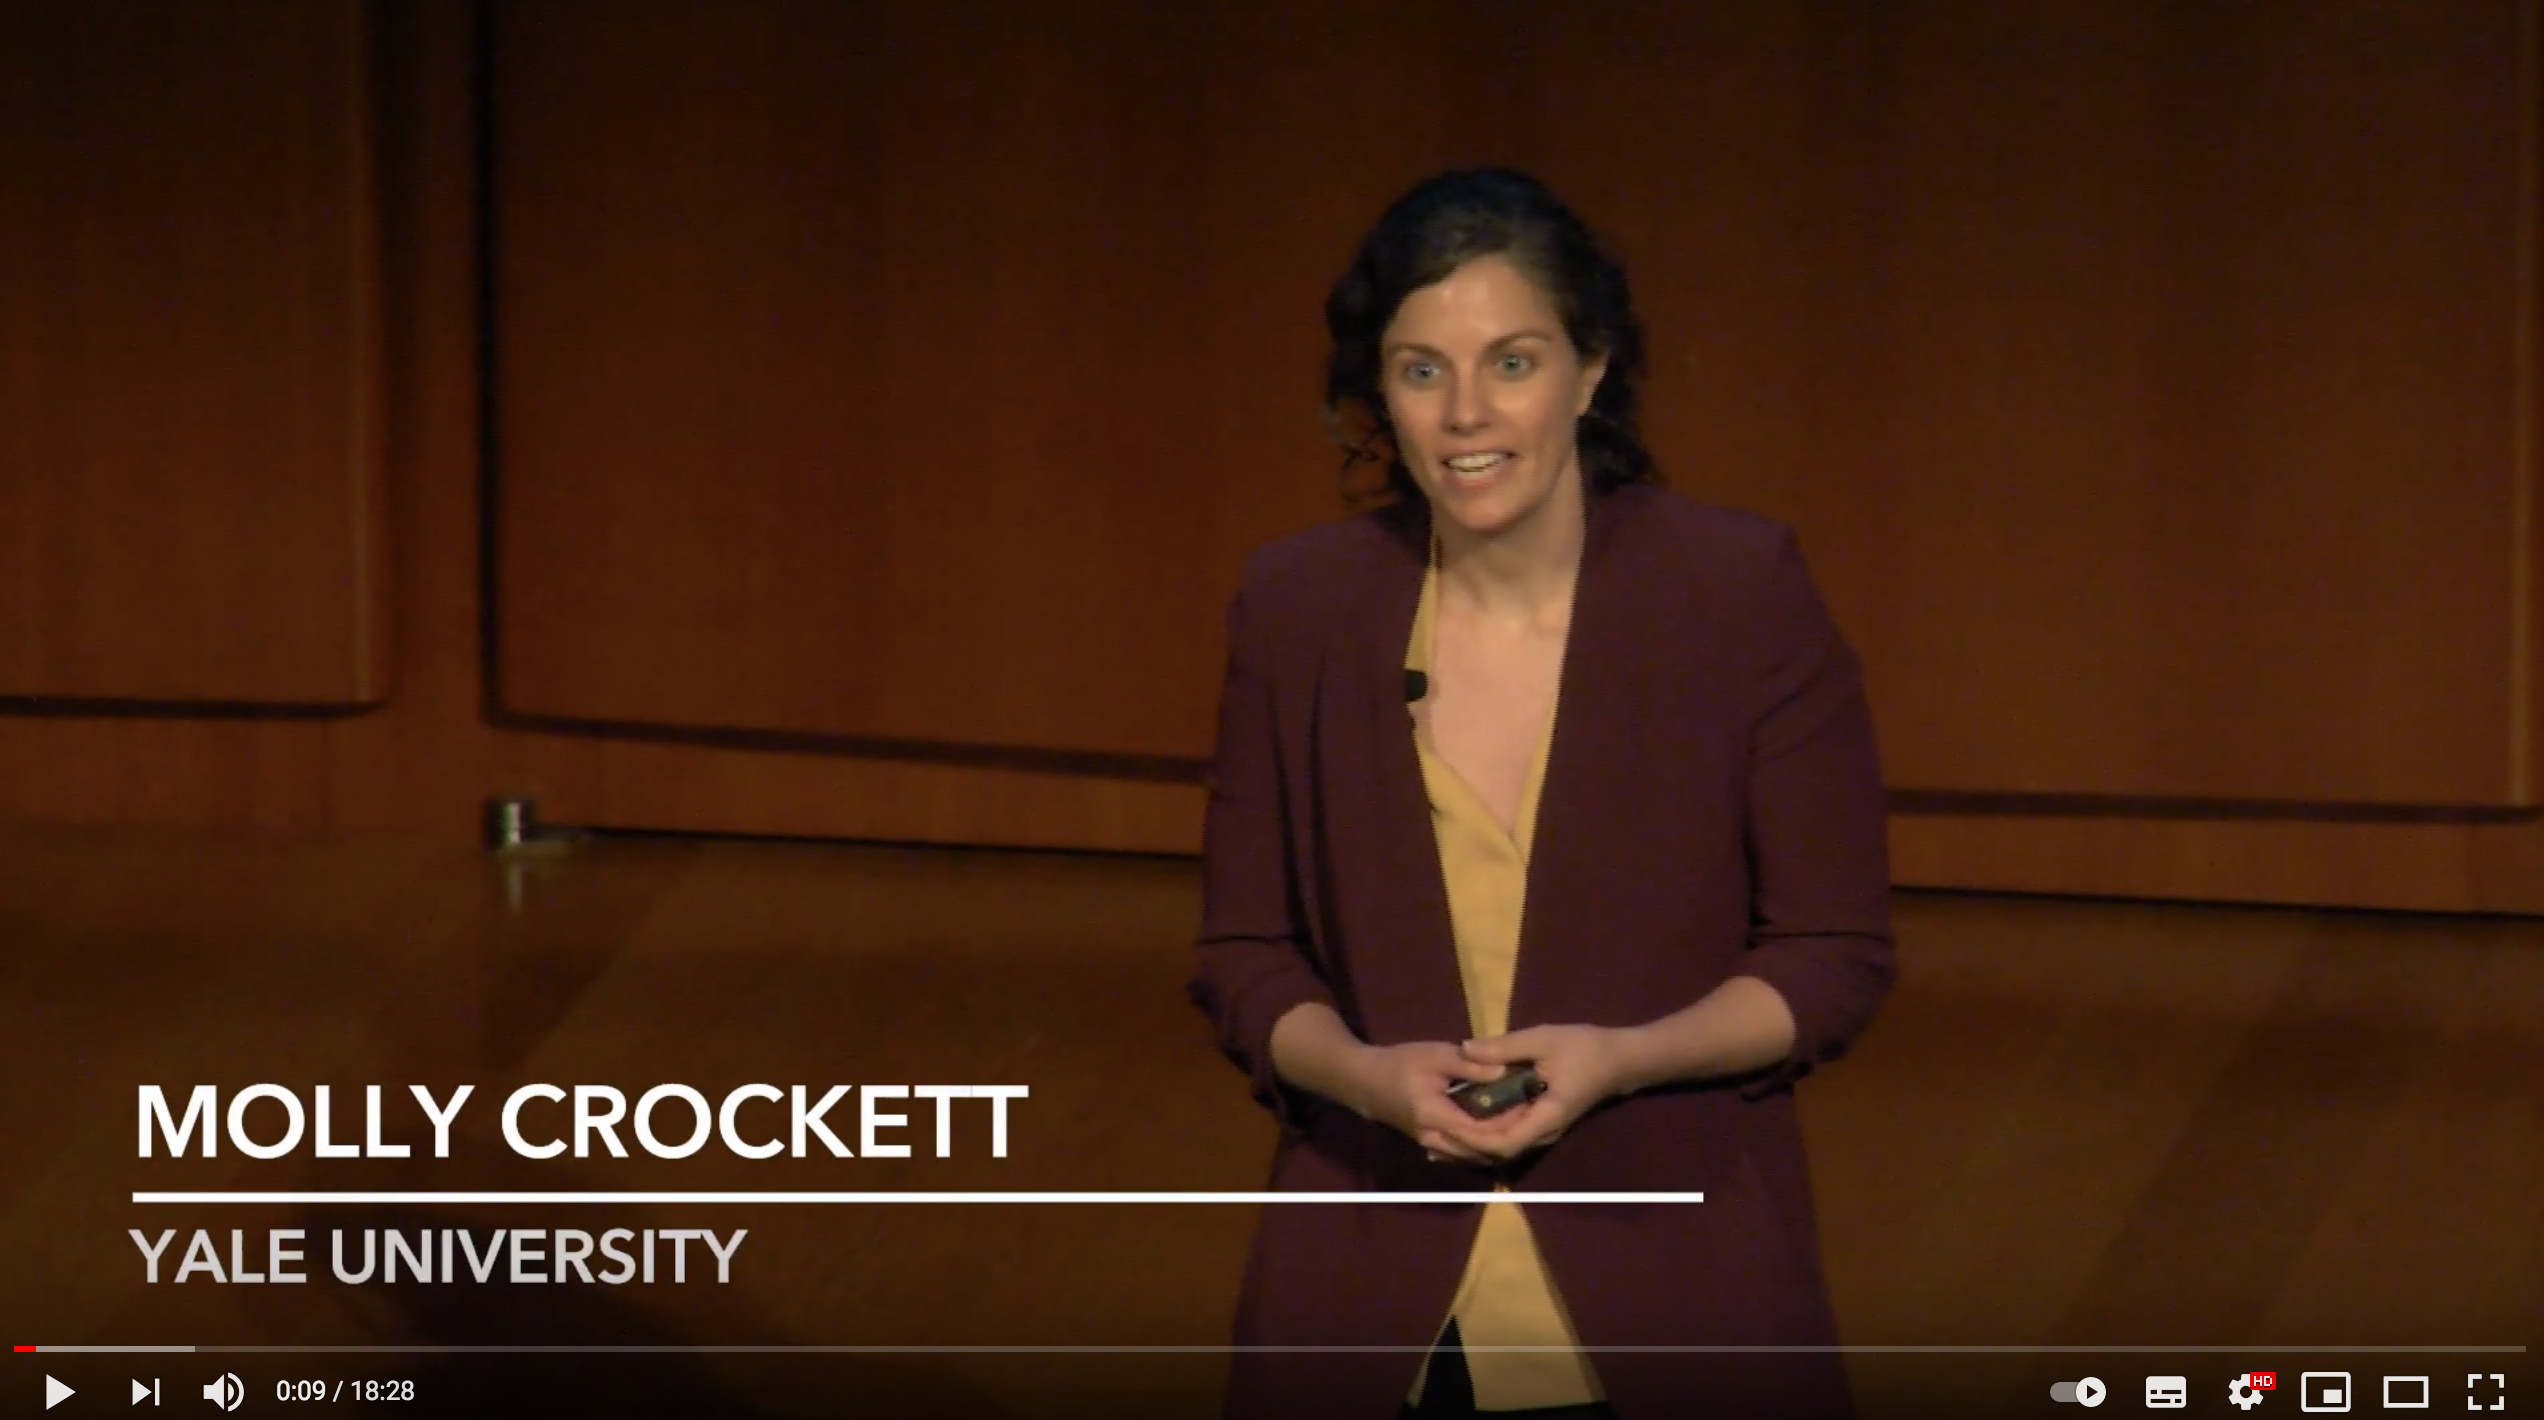
\includegraphics[width=0.95\textwidth]{figures/crockett_talk}
\end{center}

\vfill

\url{https://www.youtube.com/watch?v=b2AYlD8ReeA&t=11m26s}

\end{frame}
%%%%%%%%%%%%%%%%%%%%%%%%%
\begin{frame} 

\begin{center}
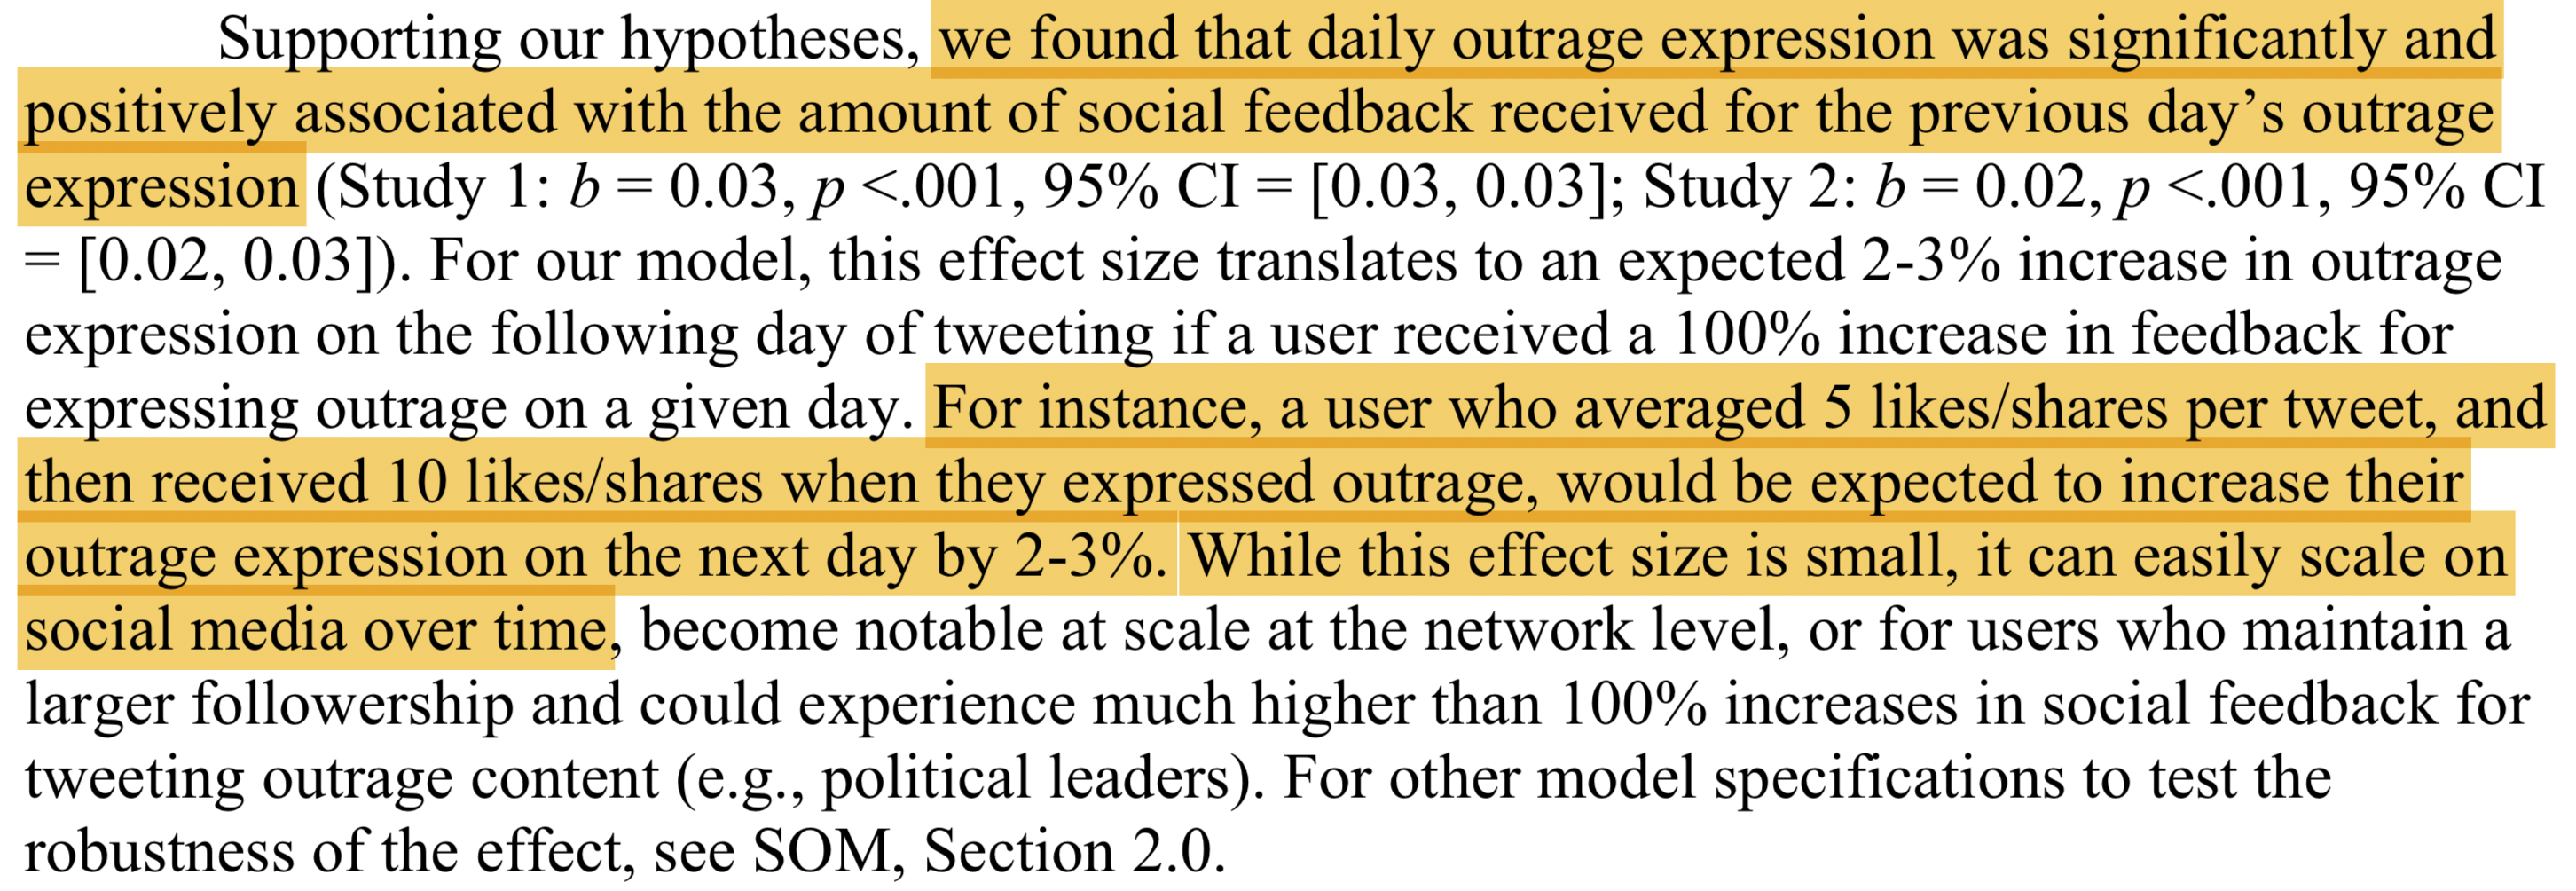
\includegraphics[width=\textwidth]{figures/brady_how_2021_study1_2}
\end{center}

\end{frame}
%%%%%%%%%%%%%%%%%%%%%%%
\begin{frame} 

Three main findings from observational studies
\begin{itemize}
\item ``outrage expression on Twitter can be explained in part by variation in social feedback that people receive via the platform'' \pause
\item ``users are more likely to express outrage in more ideologically extreme social networks'' \pause
\item ``in more ideologically extreme social networks, users' outrage expression behavior is less sensitive to social feedback.''
\end{itemize}

\vfill
Finding are consistent with reinforcement learning and norm learning, but there are limits to what they can learn just from watching without controlling the environment

\end{frame}
%%%%%%%%%%%%%%%%%%%%%%%%%%%%%%
\begin{frame}

\begin{center}
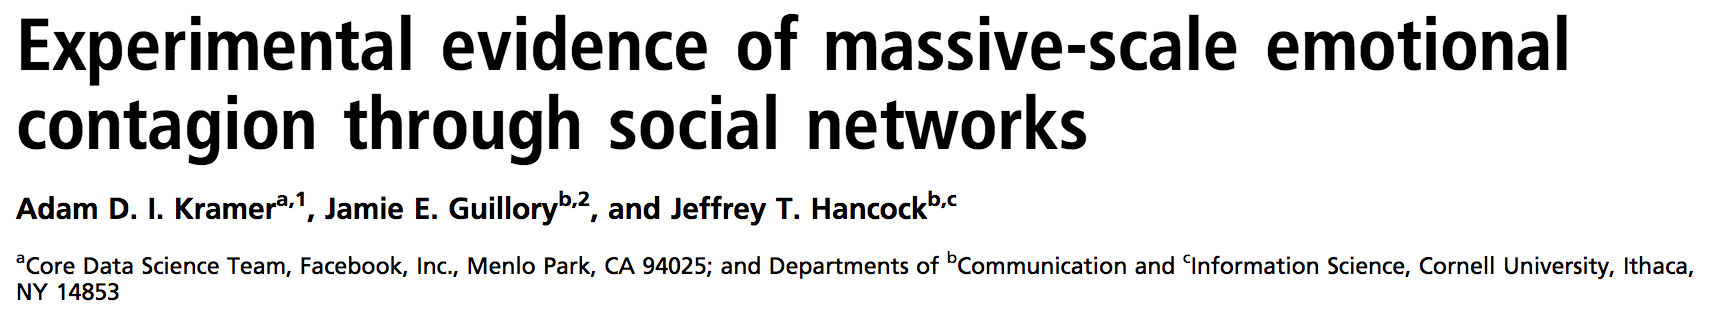
\includegraphics[width=\textwidth]{figures/kramer_experimental_2014_title}
\end{center}

\vfill

\begin{center}
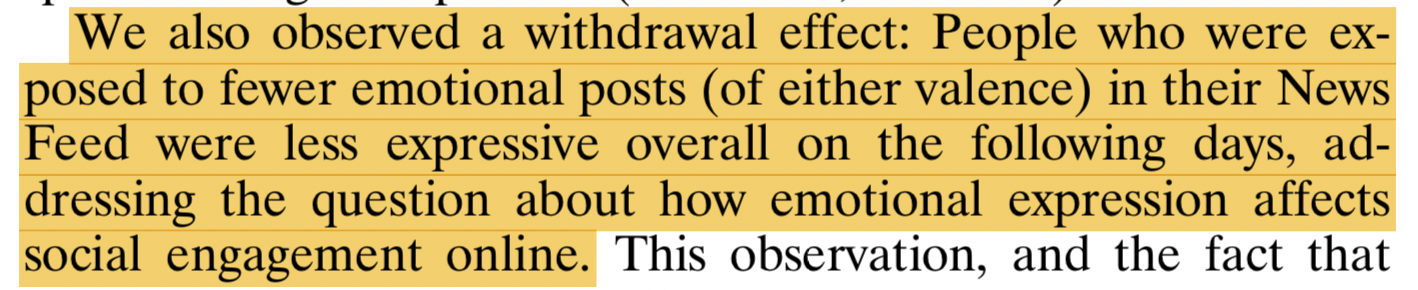
\includegraphics[width=\textwidth]{figures/kramer_experimental_2014_withdraw_effect}
\end{center}

\end{frame}
%%%%%%%%%%%%%%%%%%%%%%%%%%%%
\begin{frame} 

\begin{center}
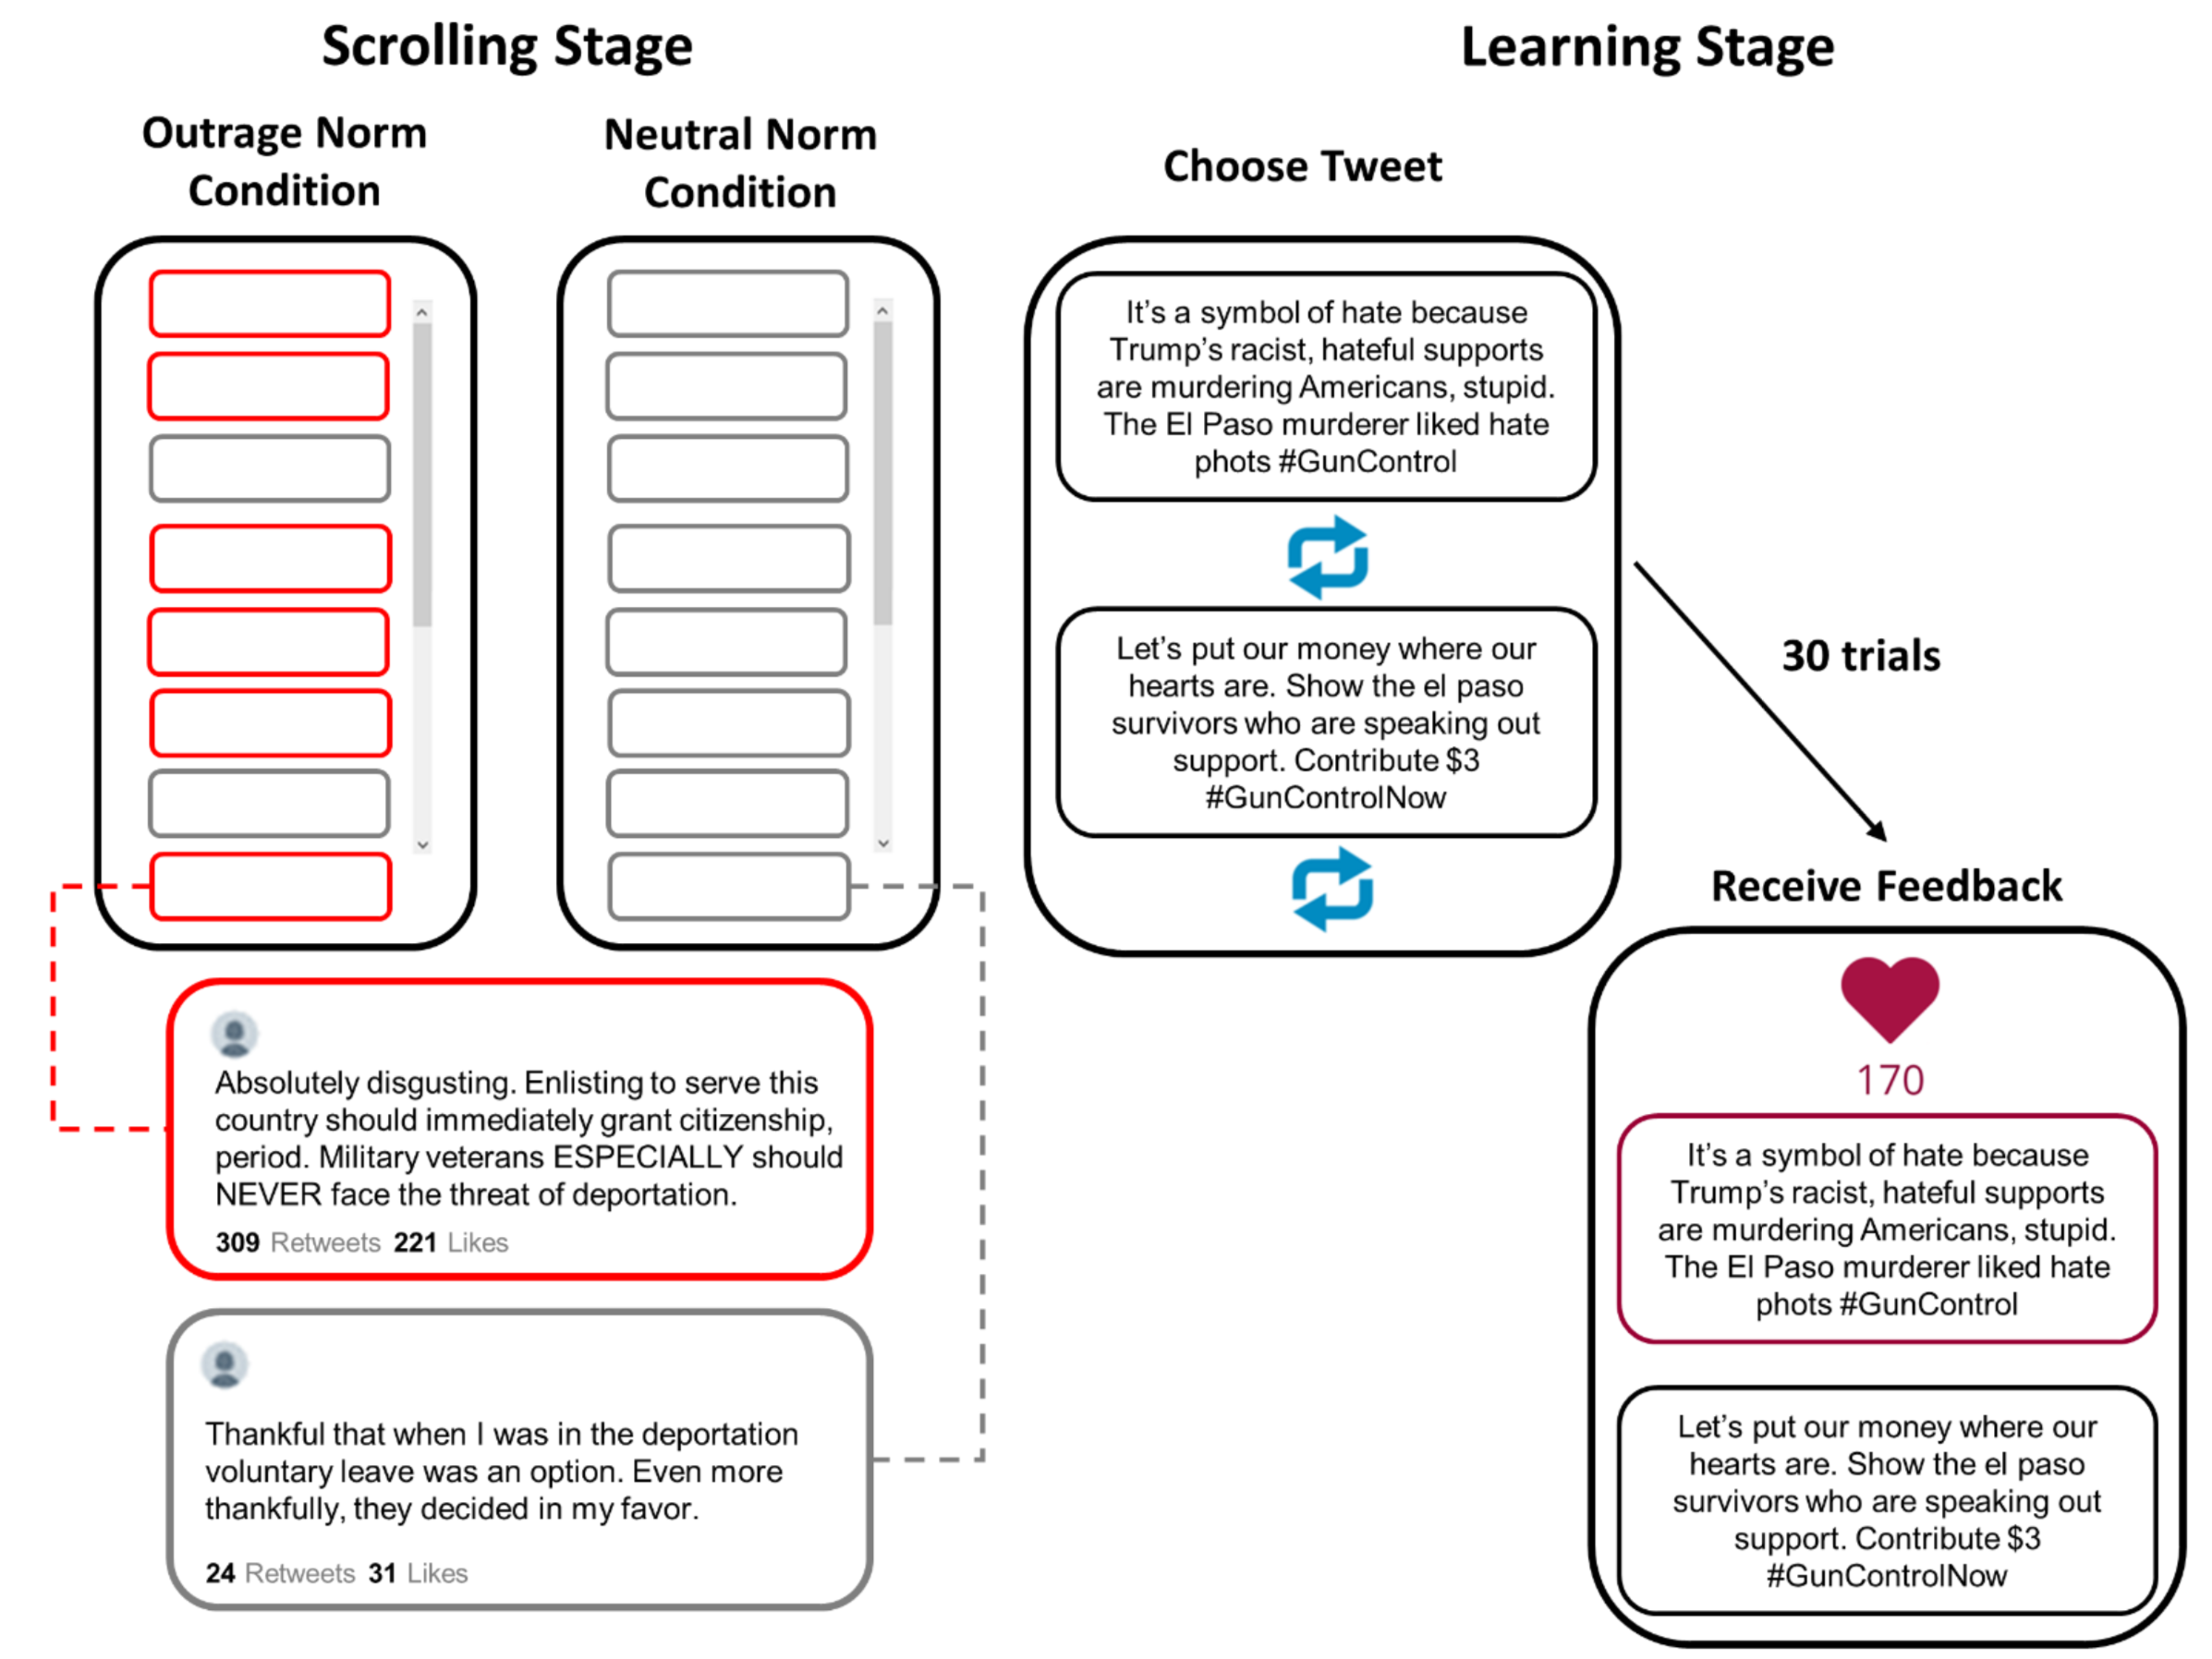
\includegraphics[height=0.8\textheight]{figures/brady_how_2021_fig3}
\end{center}

\begin{itemize}
\item Now researchers can vary the environment (norms) and feedback (reinforcement)
\end{itemize}

\end{frame}
%%%%%%%%%%%%%%%%%%%%%%%%%%%
\begin{frame} 

\begin{center}
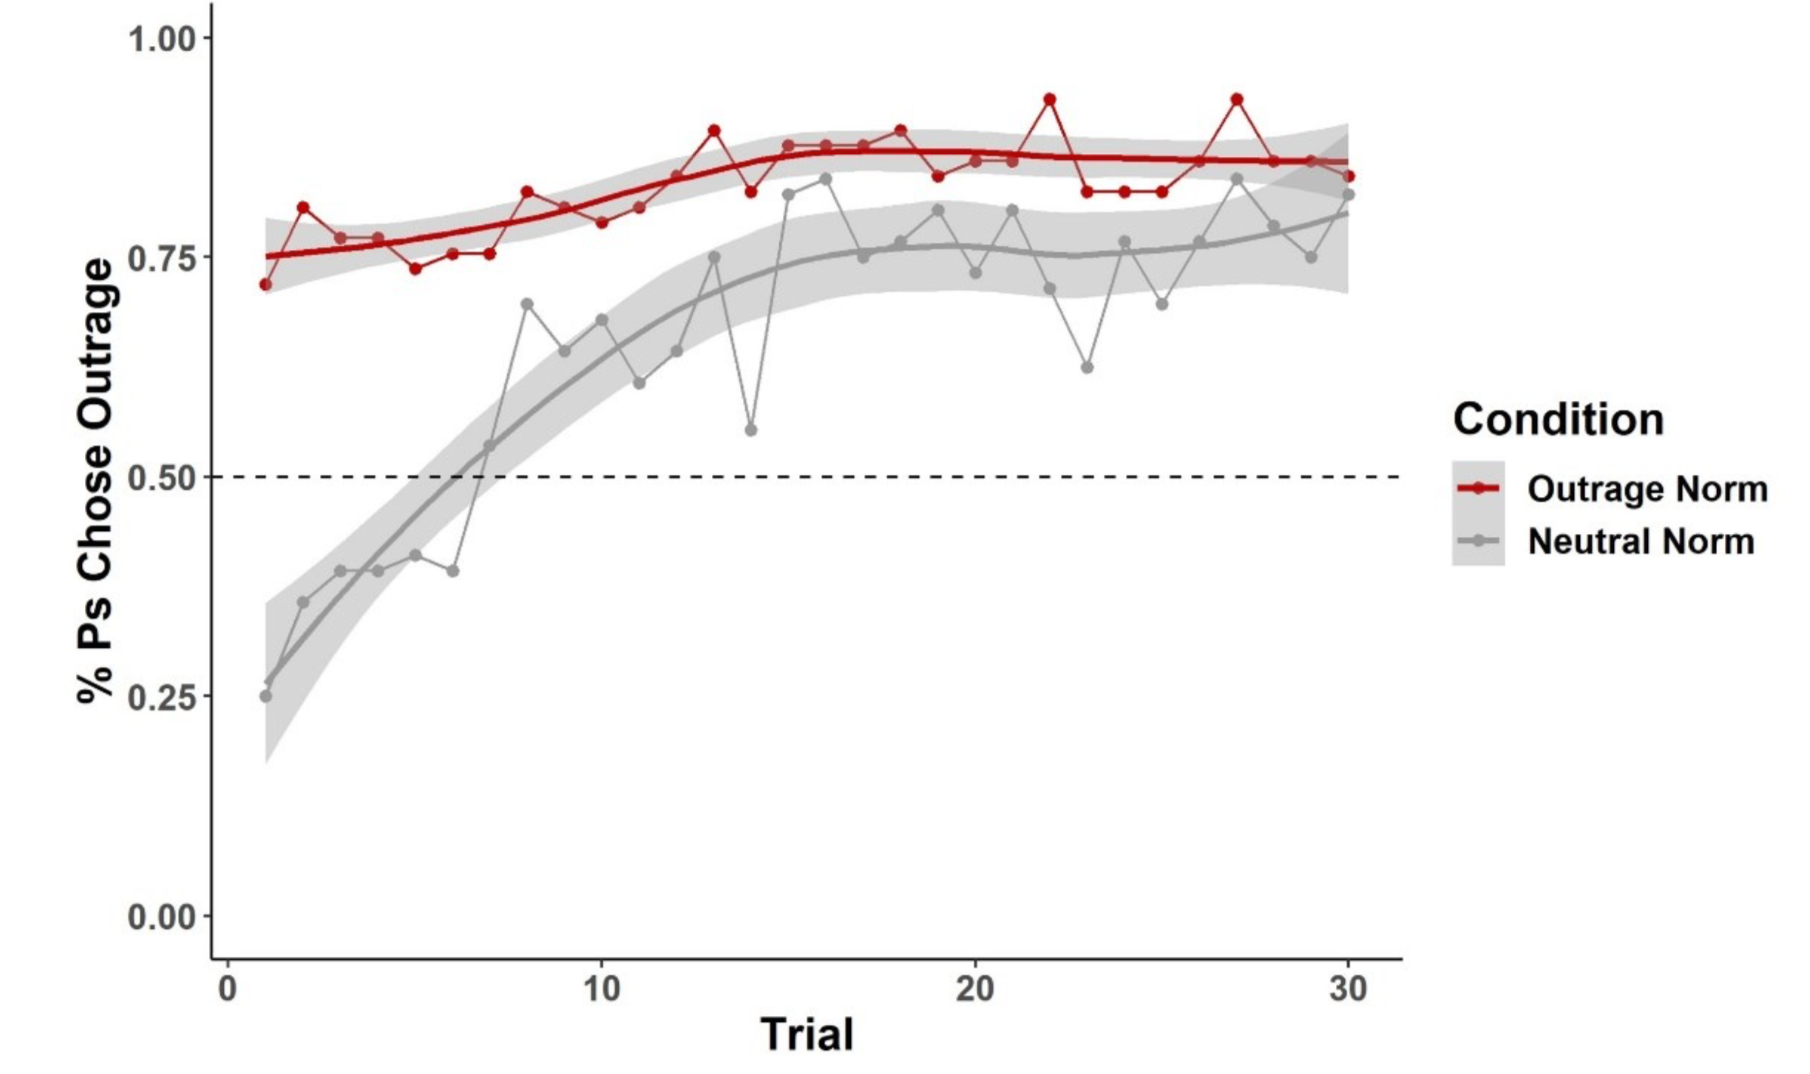
\includegraphics[width=0.8\textwidth]{figures/brady_how_2021_fig4a}
\end{center}

\begin{itemize}
\item Norms matter and people learn to choose outrage
\end{itemize}

\end{frame}
%%%%%%%%%%%%%%%%%%%%%%%%%%%
\begin{frame} 

Who is responsible?  People are doing it, but what about the architects?

\end{frame}
%%%%%%%%%%%%%%%%%%%%%%%%%%
\begin{frame}

What goes viral? Moral outrage and lies

\end{frame}
%%%%%%%%%%%%%%%%%%%%%%%%%

\begin{frame} 

\begin{center}
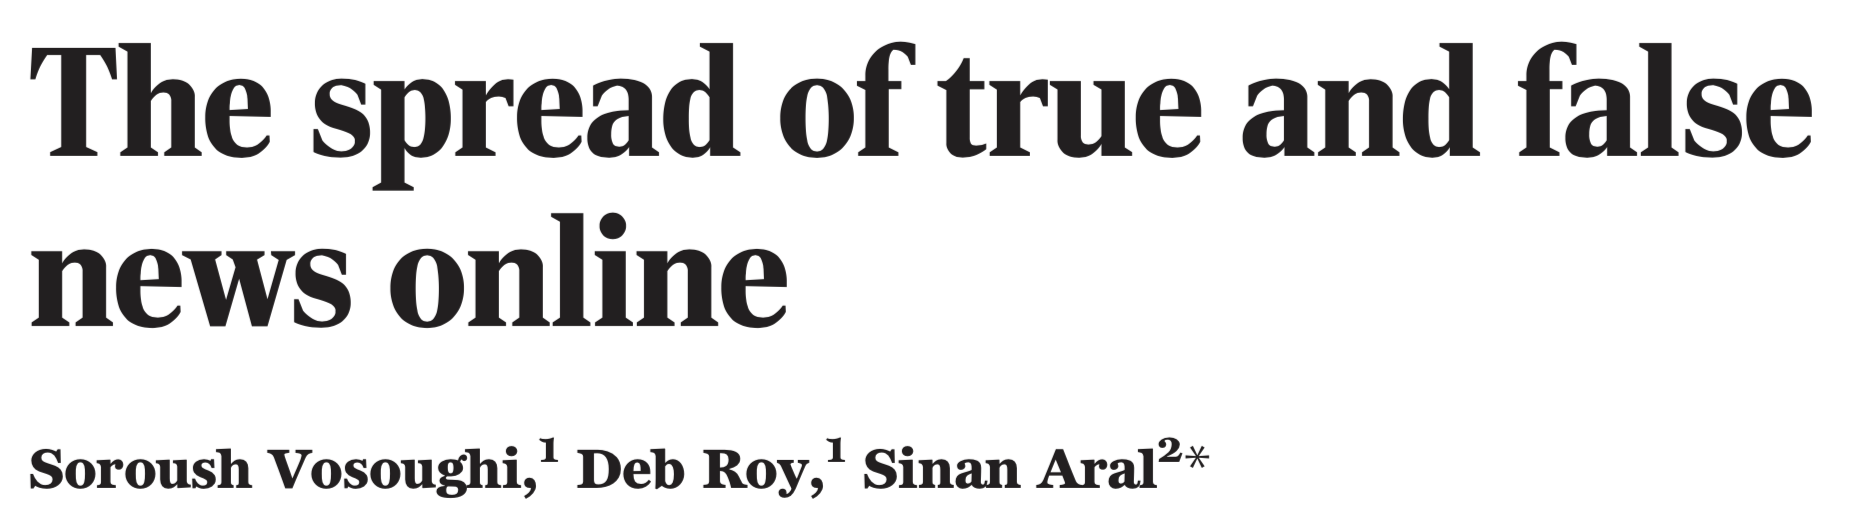
\includegraphics[width=\textwidth]{figures/vosoughi_spread_2018_title}
\end{center}

\end{frame}
%%%%%%%%%%%%%%%%%%%%%%%%%%%
\begin{frame} 

\begin{center}
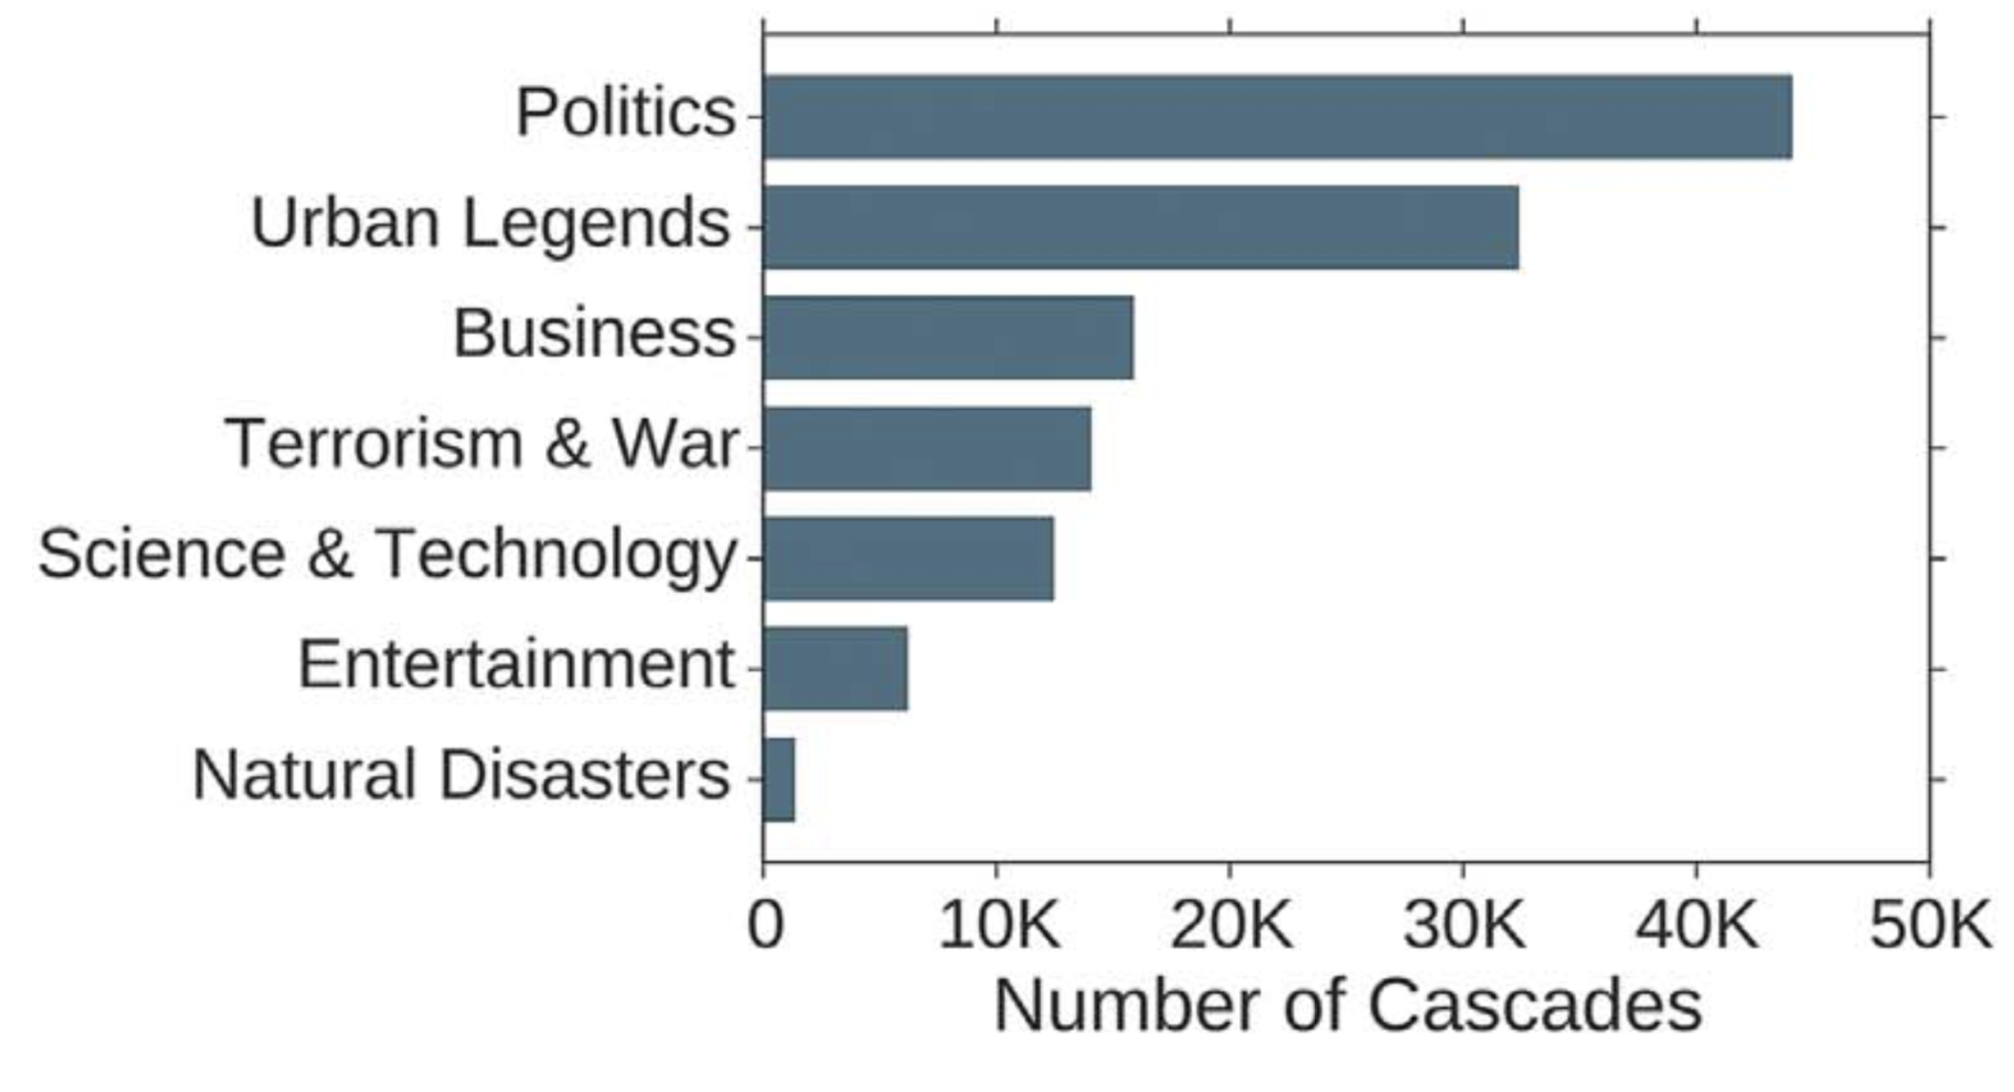
\includegraphics[width=0.9\textwidth]{figures/vosoughi_spread_2018_fig1f}
\end{center}

Unlike Goel et al.\ these are measured as true or false based on 6 fact checking websites

\end{frame}
%%%%%%%%%%%%%%%%%%%%%%%%%%%
\begin{frame} 

\begin{center}
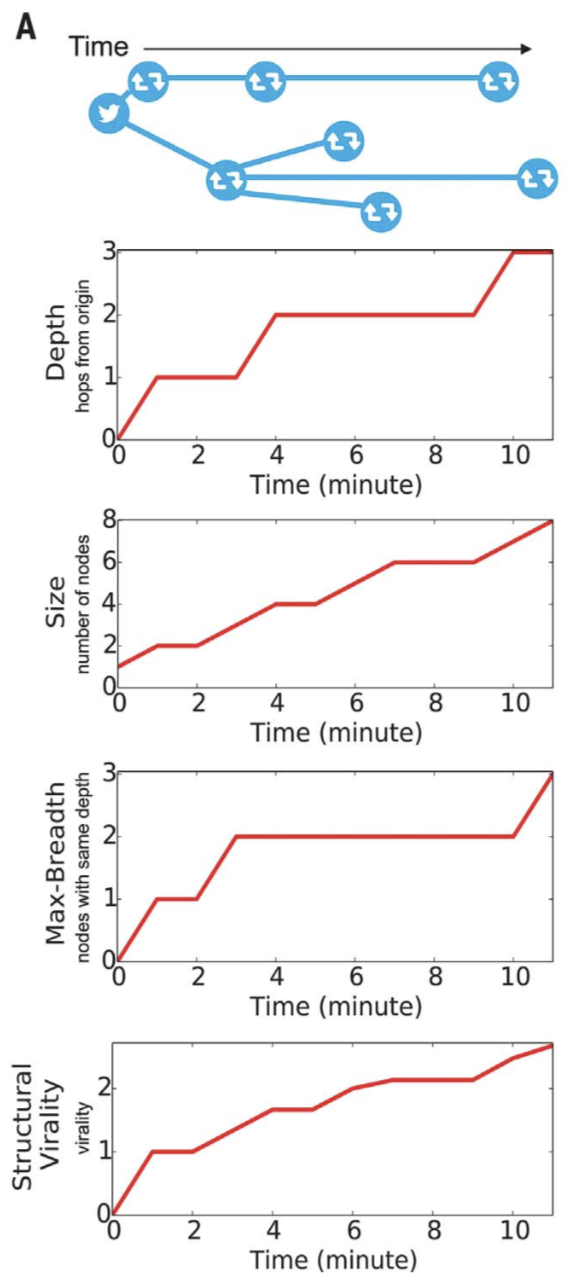
\includegraphics[height=0.9\textheight]{figures/vosoughi_spread_2018_fig1a}
\end{center}

\end{frame}
%%%%%%%%%%%%%%%%%%%%%%%%%%%
\begin{frame} 

\begin{center}
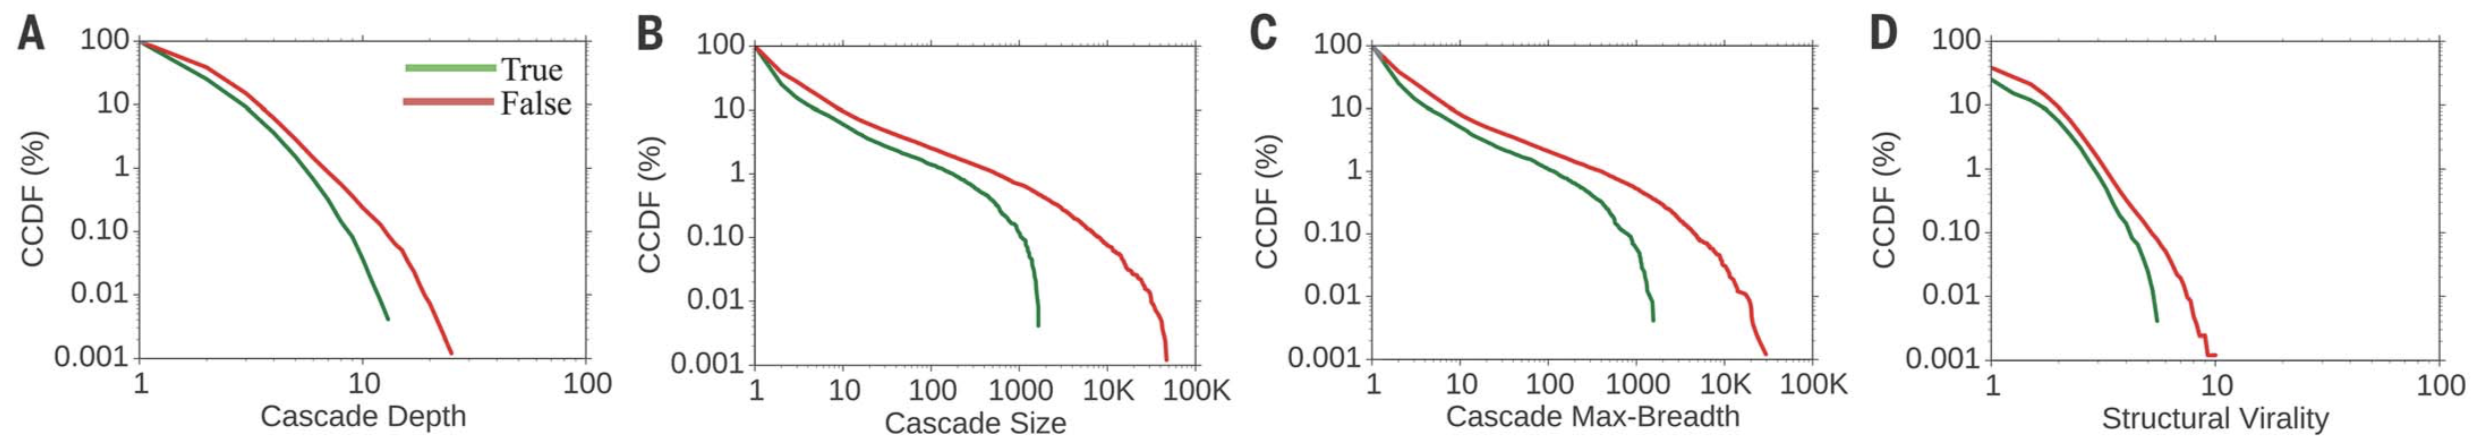
\includegraphics[width=\textwidth]{figures/vosoughi_spread_2018_fig2ad}
\end{center}

\begin{itemize}
\item false rumors spread deeper, are more retweeted, spread more broadly, and are more viral than true rumors
\end{itemize}

\end{frame}
%%%%%%%%%%%%%%%%%%%%%%%%%%%
\begin{frame} 

What might explain this pattern?  \pause False rumors are more novel than true rumors and so people decide to retweet them.

\end{frame}
%%%%%%%%%%%%%%%%%%%%%%%%%%
\begin{frame} 

\begin{itemize}
\item Is this because the face checked rumors are somehow different? \pause No. Newly, independently checked rumors show similar pattern. \pause
\item Is this because of bots? \pause No. If you remove bots you get similar patterns \pause
\item Why does this matter? \pause It impacts which policy you might use to intervene (e.g., labeling for humans, training for humans vs bot removal)
\end{itemize}

\end{frame}
%%%%%%%%%%%%%%%%%%%%%%%%%%%
\begin{frame} 

\begin{center}
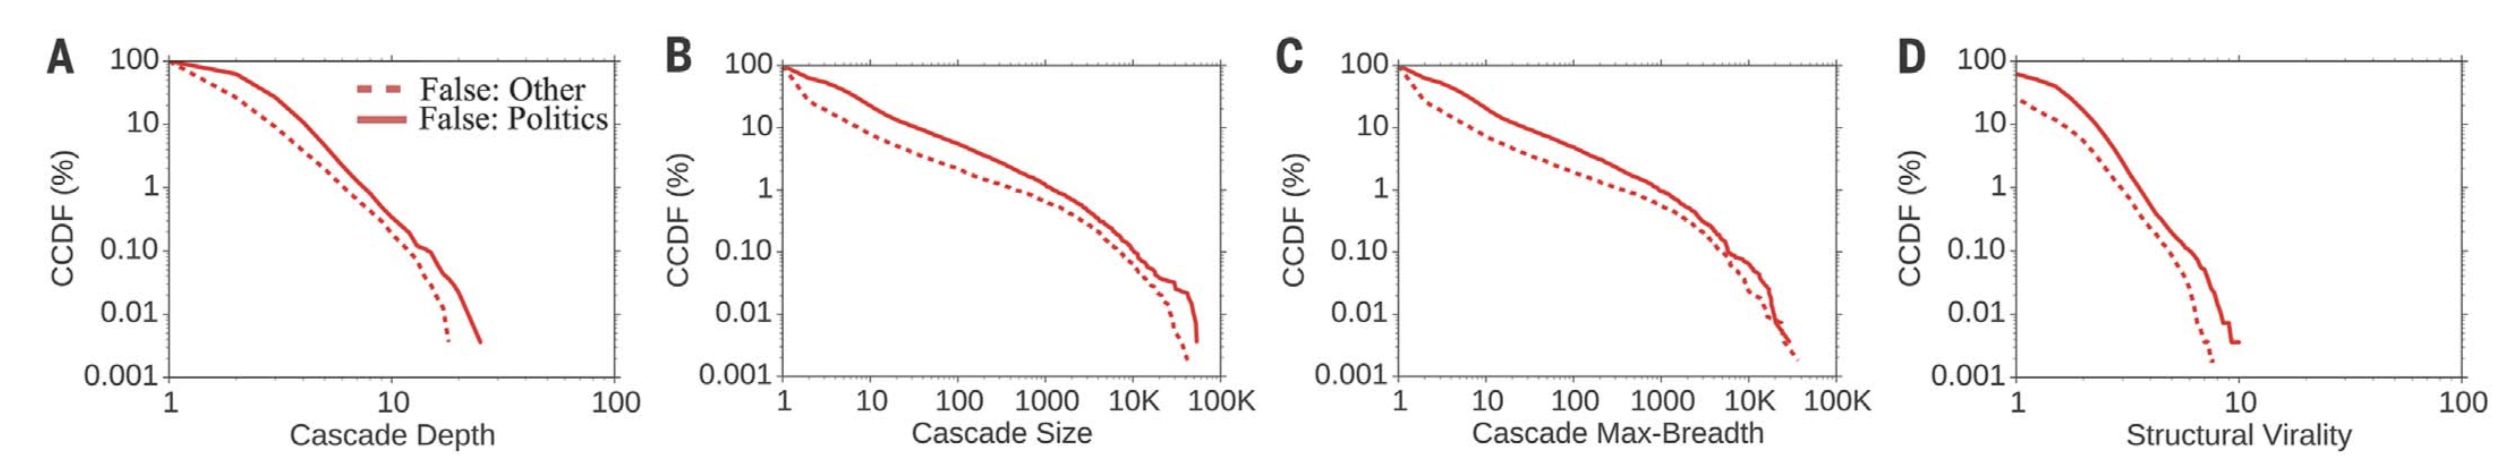
\includegraphics[width=\textwidth]{figures/vosoughi_spread_2018_fig3ad}
\end{center}

\begin{itemize}
\item political rumors spreads deeper, are more retweeted, spread more broadly, and are more viral than true rumors
\end{itemize}

\end{frame}
%%%%%%%%%%%%%%%%%%%%%%%%%%%
\begin{frame} 

All of this might make you think that we are awash in false rumors about politics, but. . . . .

\end{frame}
%%%%%%%%%%%%%%%%%%%%%%%%%%%
\begin{frame} 

\begin{center}
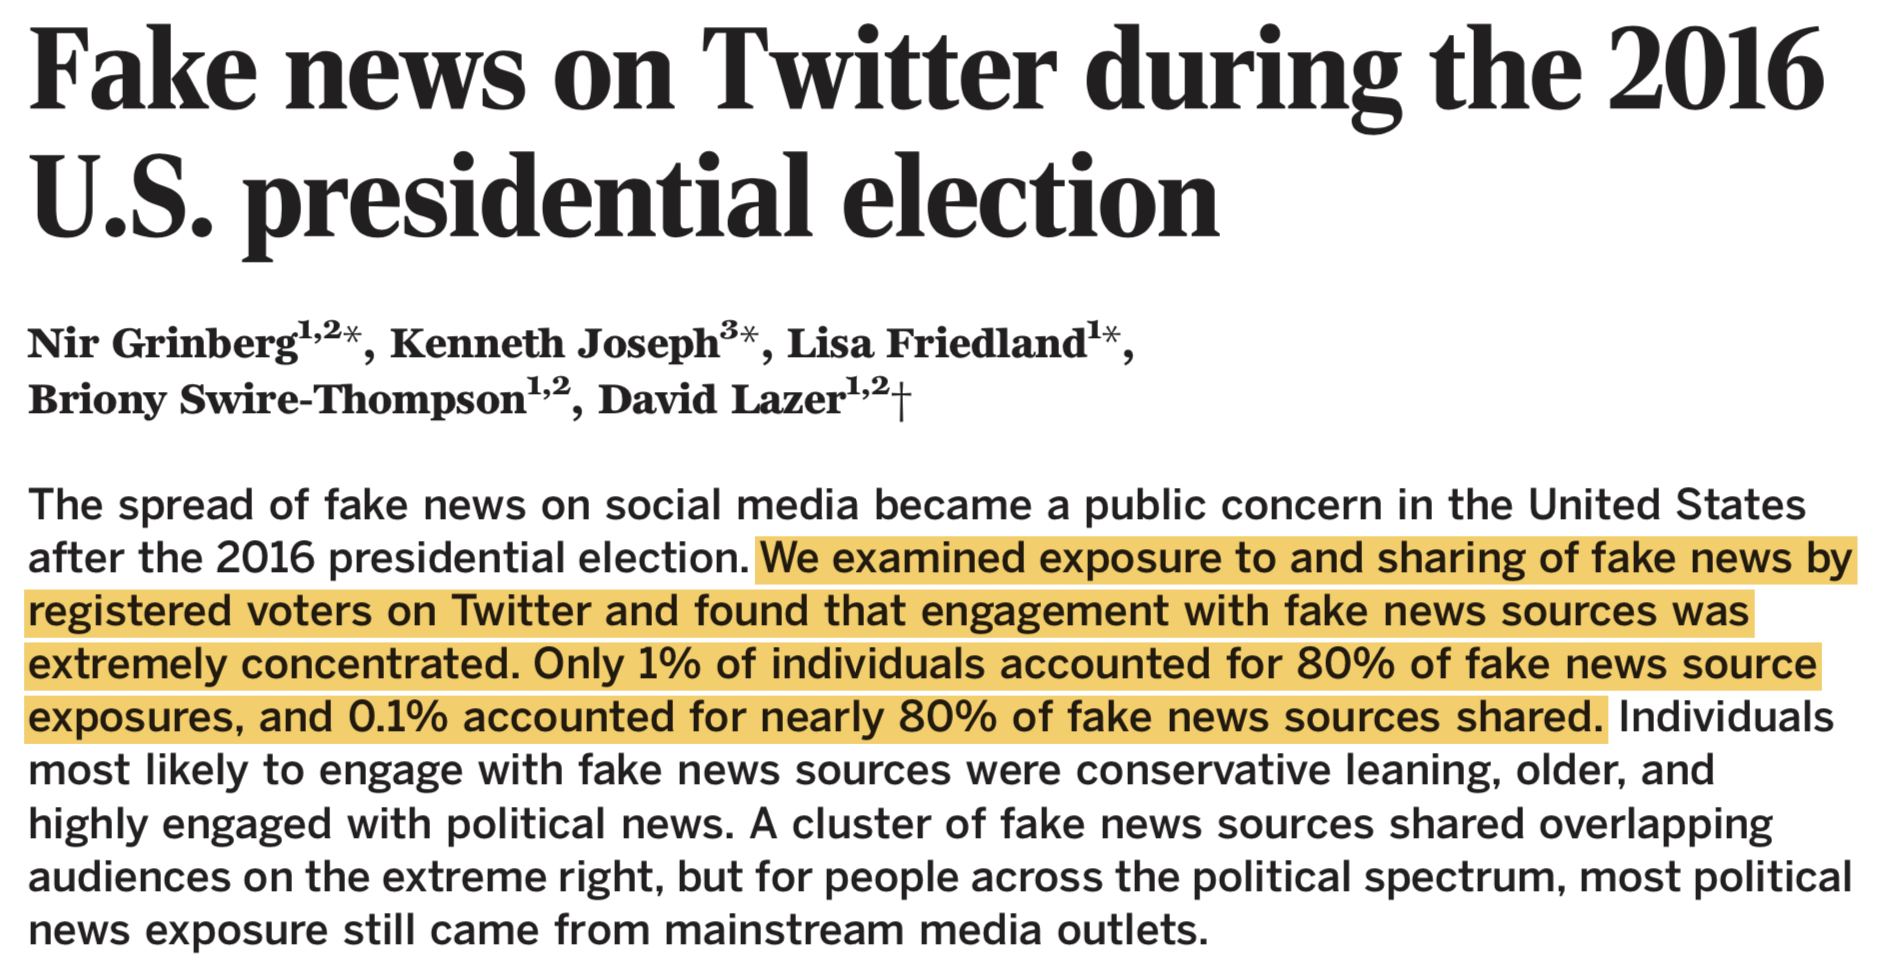
\includegraphics[width=\textwidth]{figures/grinberg_fake_2019_titleabstract}
\end{center}

\vfill
Twitter, 2016 US election, \url{https://dx.doi.org/10.1126/science.aau2706}

\end{frame}
%%%%%%%%%%%%%%%%%%%%%%%%%%%
\begin{frame} 

\begin{center}
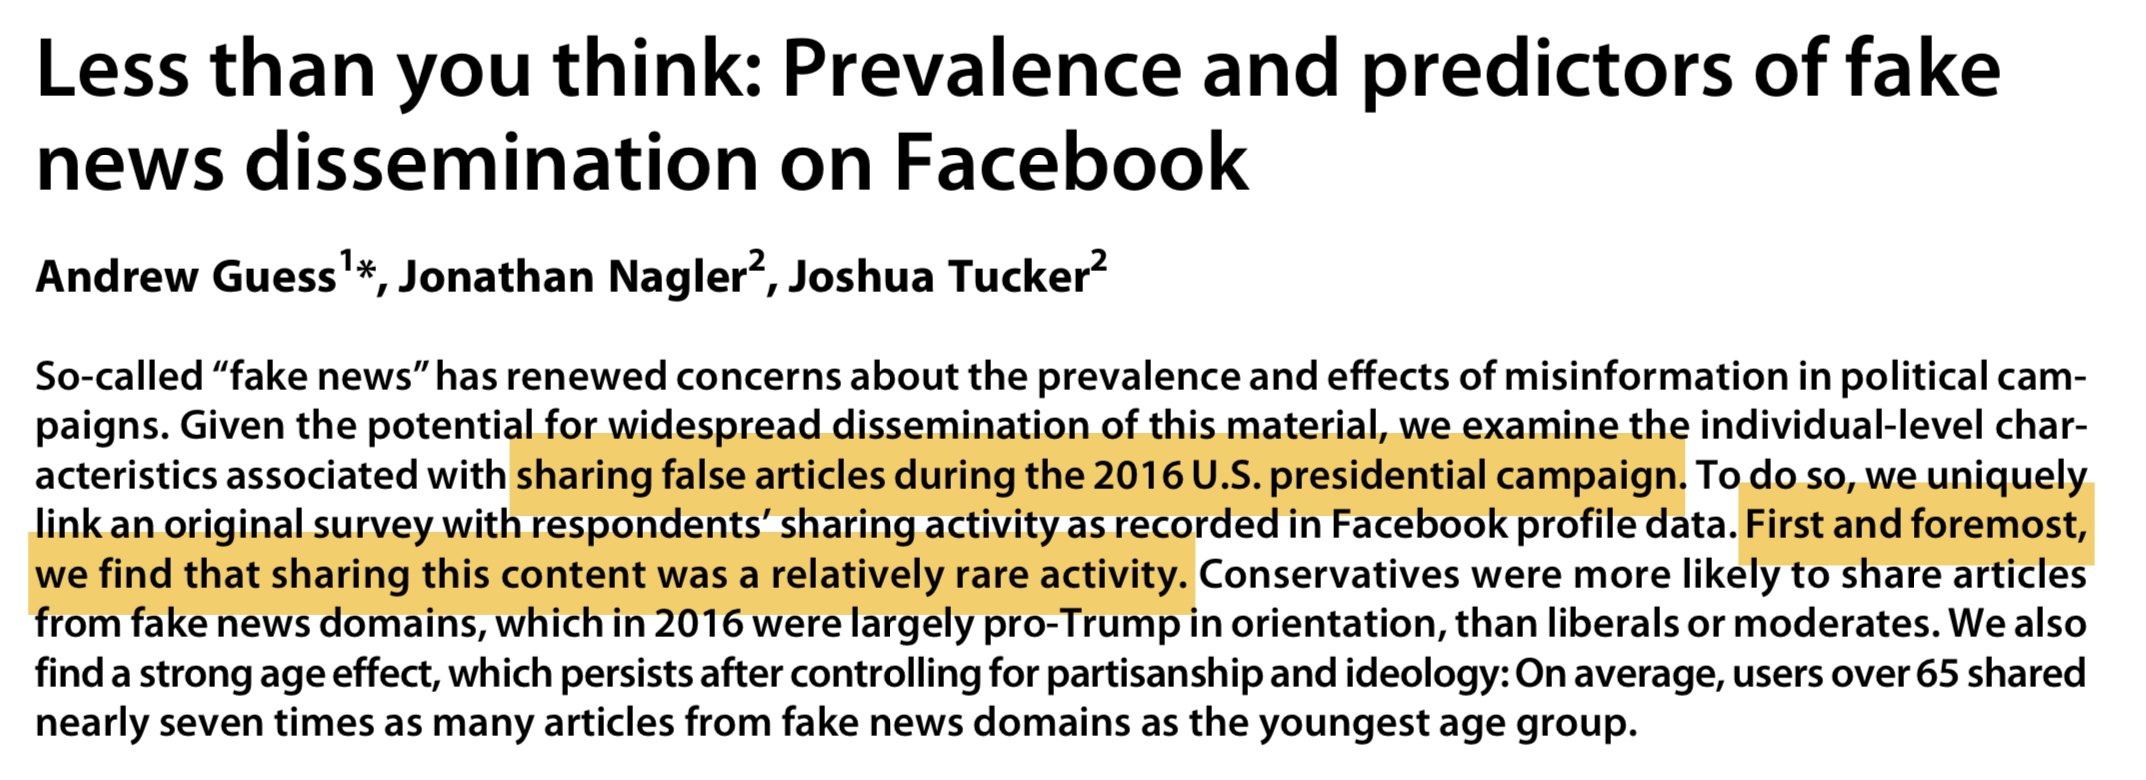
\includegraphics[width=\textwidth]{figures/guess_less_2019_titleabstract}
\end{center}

\vfill
Facebook, 2016 US election, \url{https://dx.doi.org/10.1126/sciadv.aau4586}

\end{frame}
%%%%%%%%%%%%%%%%%%%%%%%%%%%
\begin{frame} 

\begin{center}
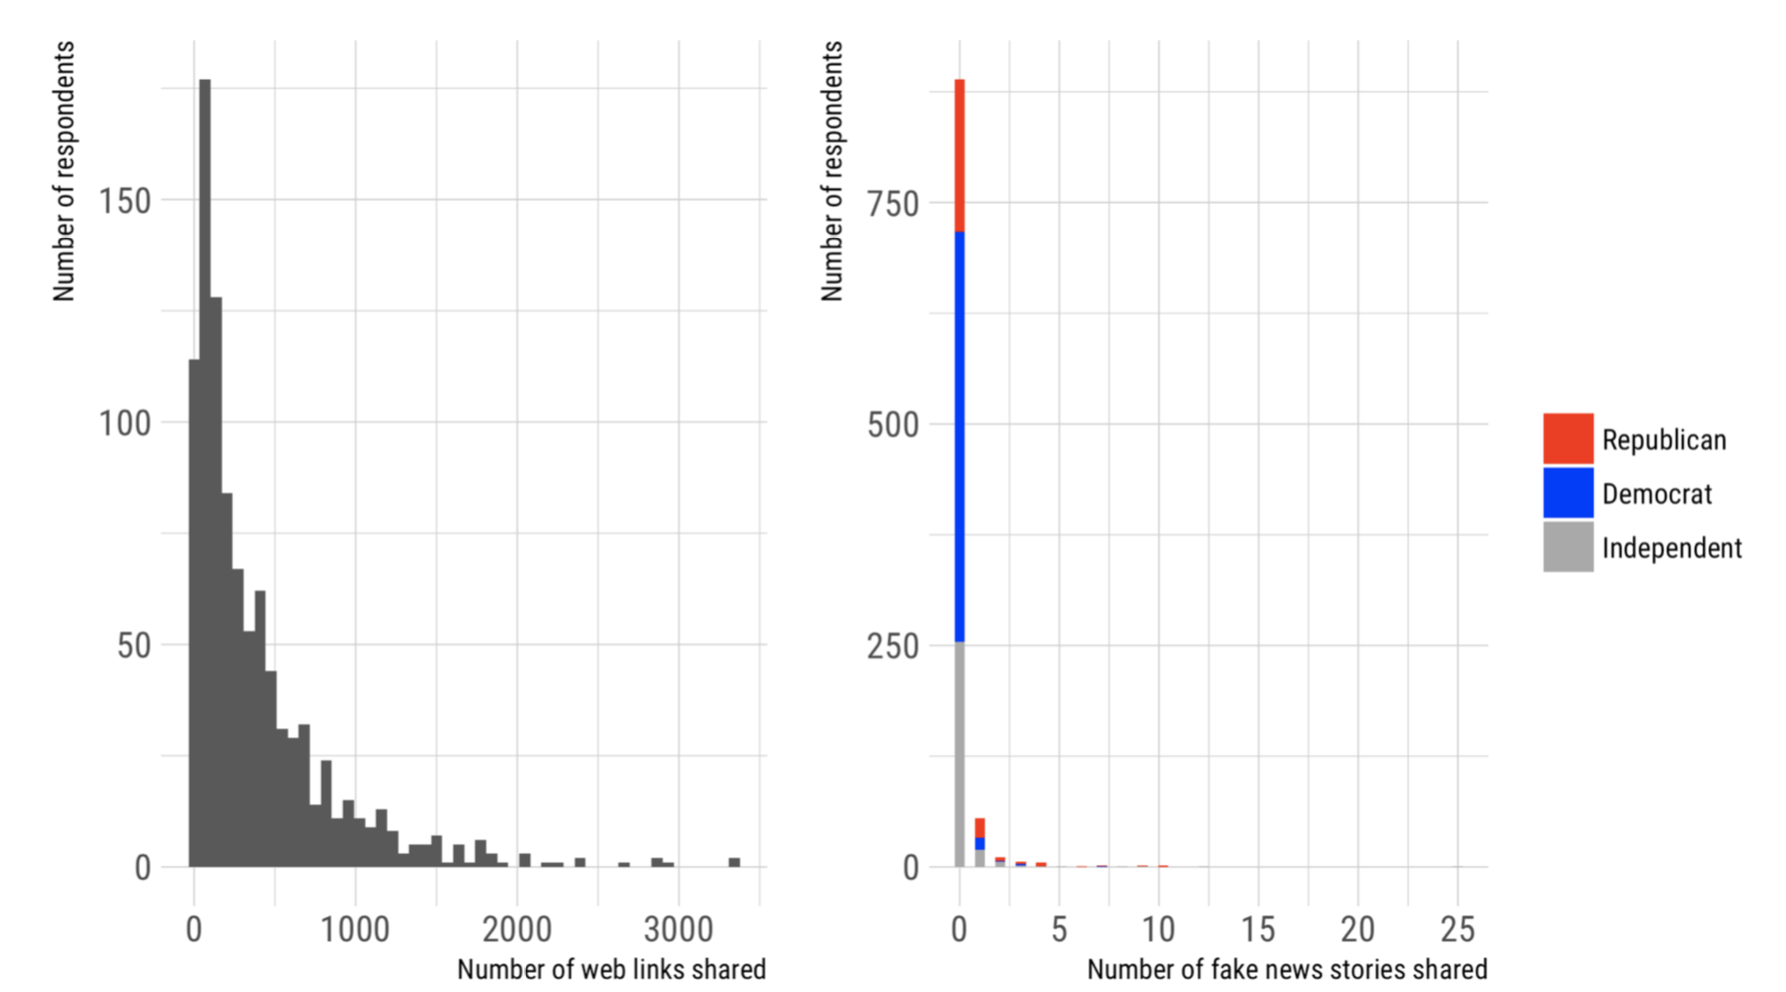
\includegraphics[width=0.9\textwidth]{figures/guess_less_2019_fig1}
\end{center}

\begin{itemize}
\item people share links of Facebook, just not fake news
\end{itemize}

\end{frame}
%%%%%%%%%%%%%%%%%%%%%%%%%%%
\begin{frame} 

Also, we have no good estimates (that I've seen) about the \emph{impact} of any of these false rumors on people's beliefs

\end{frame}
%%%%%%%%%%%%%%%%%%%%%%%%%%%
\begin{frame}

\begin{center}
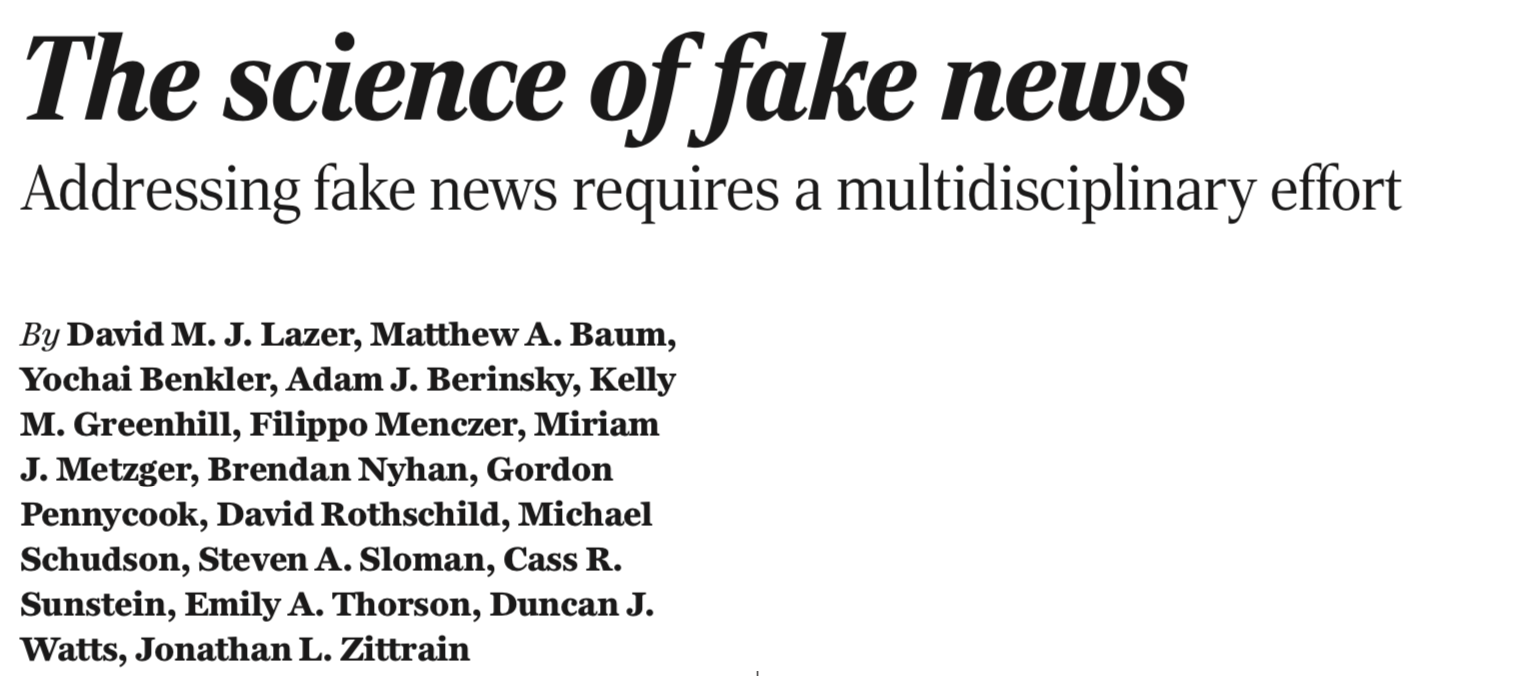
\includegraphics[width=\textwidth]{figures/lazer_science_2018_title}
\end{center}

\url{https://dx.doi.org/10.1126/science.aao2998}

\end{frame}
%%%%%%%%%%%%%%%%%%%%%%%%%%
\begin{frame}

Next lets focus on one specific algorithm thought to be related to political polarization: Facebook NewsFeed

\end{frame}

\end{document}
